% autosam.tex
% Annotated sample file for the preparation of LaTeX files
% for the final versions of papers submitted to or accepted for 
% publication in AUTOMATICA.

% See also the Information for Authors.

% Make sure that the zip file that you send contains all the 
% files, including the files for the figures and the bib file.

% Output produced with the elsart style file does not imitate the
% AUTOMATICA style. The style file is generic for all Elsevier
% journals and the output is laid out for easy copy editing. The
% final document is produced from the source file in the
% AUTOMATICA style at Elsevier.

% You may use the style file autart.cls to obtain a two-column 
% document (see below) that more or less imitates the printed 
% Automatica style. This may helpful to improve the formatting 
% of the equations, tables and figures, and also serves to check 
% whether the paper satisfies the length requirements.

% Please note: Authors must not create their own macros.

% For further information regarding the preparation of LaTeX files 
% for Elsevier, please refer to the "Full Instructions to Authors" 
% from Elsevier's anonymous ftp server on ftp.elsevier.nl in the
% directory pub/styles, or from the internet (CTAN sites) on
% ftp.shsu.edu, ftp.dante.de and ftp.tex.ac.uk in the directory
% tex-archive/macros/latex/contrib/supported/elsevier.


%\documentclass{elsart}               % The use of LaTeX2e is preferred.

\documentclass[twocolumn]{autart}    % Enable this line and disable the 
                                     % preceding line to obtain a two-column 
                                     % document whose style resembles the
                                     % printed Automatica style.


\usepackage{graphicx}          % Include this line if your 
                               % document contains figures,
%\usepackage[dvips]{epsfig}    % or this line, depending on which
                               % you prefer.

% ===================================================================
\usepackage{amsmath}
\usepackage{amsfonts}
\usepackage[nolist]{acronym}    % required for \acro

\usepackage[textsize=tiny]{todonotes}
\usepackage{tikz,ifthen}
\usetikzlibrary{calc}

% own definitions:
\newcommand{\eqnref}[1]{(\ref{#1})}
\newcommand{\figref}[1]{Fig.~\ref{#1}}
\newcommand{\secref}[1]{Section~\ref{#1}}
\newcommand{\inv}{^{\raisebox{.2ex}{$\scriptscriptstyle-1$}}}
\newcommand{\Tf}[1]{\mathcal{T}_f^\mathrm{{#1}}}
\newcommand{\tTf}[1]{\widetilde{\mathcal{T}}_f^\mathrm{{#1}}}
\newcommand{\hTf}[1]{\widehat{\mathcal{T}}_f^\mathrm{{#1}}}
\newcommand{\Hf}{\mathcal{H}_f}
\newcommand{\tHf}{\widetilde{\mathcal{H}}_f}
\newcommand{\hHf}{\widehat{\mathcal{H}}_f}
\newcommand{\Kp}[1]{\mathcal{K}_{p}^{\mathrm{{#1}}}}
\newcommand{\tKp}[1]{\widetilde{\mathcal{K}}_{p}^{\mathrm{{#1}}}}
\newcommand{\Gf}{\Gamma_f}
\newcommand{\tGf}{\widetilde{\Gamma}_f}
\newcommand{\datavec}[2]{\underline{#1}_{#2}} % <-- add own preamble stuff
% ===================================================================

\begin{document}

\begin{frontmatter}
%\runtitle{Insert a suggested running title}  % Running title for regular 
                                              % papers but only if the title  
                                              % is over 5 words. Running title 
                                              % is not shown in output.

\title{Closed-loop Data-Enabled Predictive Control\thanksref{footnoteinfo}} % Title, preferably not more 
                                                % than 10 words.

\thanks[footnoteinfo]{This paper was not presented at any IFAC meeting.}
% \corauth[cor1]{Corresponding author.% R.~Dinkla. Tel. +XXXIX-VI-mmmxxi. Fax +XXXIX-VI-mmmxxv.
% }

\author[TUD]{R. Dinkla\corauthref{cor}}\ead{r.t.o.dinkla@tudelft.nl},    % Add the
\corauth[cor]{Corresponding author.% R.~Dinkla. Tel. +XXXIX-VI-mmmxxi. Fax +XXXIX-VI-mmmxxv.
}
\author[TUD]{S. P. Mulders}\ead{s.p.mulders@tudelft.nl},               % e-mail address 
\author[TUD,TUE]{T. Oomen}\ead{t.a.e.oomen@tudelft.nl},  % (ead) as shown
\author[TUD]{J.W. van Wingerden}\ead{j.w.vanwingerden@tudelft.nl}
\address[TUD]{Delft Center for Systems and Control, Delft University of Technology, Mekelweg 2, 2628CD Delft, The Netherlands}  % Please supply                                              
\address[TUE]{Control Systems Technology Group, Eindhoven University of Technology, 5600
MB Eindhoven, The Netherlands}        % Ful addresses here.

          
\begin{keyword}                           % Five to ten keywords,  
Cicero; Catiline; orations.               % chosen from the IFAC 
\end{keyword}                             % keyword list or with the 
                                          % help of the Automatica 
                                          % keyword wizard


\begin{abstract}                          % Abstract of not more than 200 words.
Cum M.~Cicero consul Nonis Decembribus senatum in aede Iovis 
Statoris consuleret, quid de iis coniurationis Catilinae sociis 
fieri placeret, qui in custodiam traditi essent, factum est, ut 
duae potissimum sententiae proponerentur, una D.~Silani consulis 
designati, qui morte multandos illos censebat, altera C.~Caesaris, 
qui illos publicatis bonis per municipia Italiae distribuendos 
ac vinculis sempiternis tenendos existimabat.
Cum M.~Cicero consul Nonis Decembribus senatum in aede Iovis 
Statoris consuleret, quid de iis coniurationis Catilinae sociis 
fieri placeret, qui in custodiam traditi essent, factum est, ut 
duae potissimum sententiae proponerentur, una D.~Silani consulis 
designati, qui morte multandos illos censebat, altera C.~Caesaris, 
qui illos publicatis bonis per municipia Italiae distribuendos 
ac vinculis sempiternis tenendos existimabat.
Cum M.~Cicero consul Nonis Decembribus senatum in aede Iovis 
Statoris consuleret, quid de iis coniurationis Catilinae sociis 
fieri placeret, qui in custodiam traditi essent, factum est, ut 
duae potissimum sententiae proponerentur, una D.~Silani consulis 
designati, qui morte multandos illos censebat, altera C.~Caesaris, 
qui illos publicatis bonis per municipia Italiae distribuendos 
ac vinculis sempiternis tenendos existimabat.
\end{abstract}

\end{frontmatter}
%===============================================================================
% define acronyms here
\begin{acronym}%
    \acro{SPC}{Subspace Predictive Control}
    \acro{CL-SPC}{closed-loop Subspace Predictive Control}
    \acro{DeePC}{Data-enabled Predictive Control}
    \acro{LTI}{linear time-invariant}
    \acro{IV}{instrumental variable}
    \acro{IVs}{instrumental variables}
    \acro{N4SID}{Numerical algorithm for Subspace State Space System Identification}
    \acro{MPC}{Model Predictive Control}
    \acro{CL-DeePC}{closed-loop Data-enabled Predictive Control}
\end{acronym}%
%===============================================================================
\section{Introduction}\label{sec:introduction}
\noindent Trends of increasing data availability as well as increasing system complexity provide opportunities for data driven-driven control%make a compelling case for data-driven control methods as an alternative to model-based approaches
~\citep{Hou2013}. In sharp contrast to the use of data in %Whilst data can be used with
indirect data-driven approaches to synthesise a model by means of system identification, direct data-driven control approaches are promising because of their ability to derive a control law directly from data without having to realize an explicit system model as an often expensive intermediate step~\citep{Hjalmarsson2005}.

A direct \ac{DDPC} method called \acf{DeePC} is developed in~\cite{Coulson2019} and has recently seen considerable development and successful implementation~\cite{Markovsky2023}. \ac{DeePC} relies on Willems' Fundamental Lemma in a receding horizon optimal control framework. This lemma reveals that for a deterministic \ac{LTI} system, any sufficiently persistently exciting input-output trajectory parameterizes all possible future input-output trajectories~\citep{Willems2005}.

% Since its conception in~\cite{Coulson2019}, a form of direct data-driven control called \ac{DeePC} has seen considerable development. \ac{DeePC} uses Willems' Fundamental Lemma from the field of behavioural systems theory, which states that for a deterministic system any sufficiently persistently exciting input-output trajectory parameterizes all possible future input-output trajectories~\cite{Willems2005}. In effect, \ac{DeePC} exploits Willems' Fundamental Lemma in a receding horizon optimal control framework found also in \ac{MPC}.
For non-deterministic systems, care has to be taken with such a parameterization in terms of only past input-output trajectories because this does not consider the effects of noise. If the block-Hankel data matrix in which the noisy input-output trajectories are stored is full rank then unattainable future trajectories may be predicted~\citep{Markovsky2022}. On the other hand, if the data matrix is rank-deficient, then the \ac{DeePC} problem may be infeasible. To deal with noise, slack variables and regularization initially served as heuristic measures to introduce robustness~\citep{Coulson2019}, and subsequently have been motivated formally to, e.g., provide robust closed-loop stability guarantees~\citep{Berberich2021}, distributional robustness~\citep{Coulson2019a}, and robustness to structured uncertainty~\citep{Huang2023}. Other approaches to handle noise include averaging techniques~\citep{Jo2022}, singular value based thresholding~\citep{Sassella2022}, and the use of maximum likelihood estimation~\citep{Yin2023}. See also~\cite{Sassella2023} for a discussion of such methods, or \cite{Verheijen2023} for a practical review of several \ac{DDPC} methods.% that consider noise.

To fundamentally address the consequences of noise in a data-driven setting, an \ac{IV} approach is presented in~\cite{vanWingerden2022}. %A fundamentally different noise-mitigation technique is the use of \acf{IVs}.
Using \ac{IVs} to mitigate noise, this method %
%These are employed in~\cite{vanWingerden2022} to mitigate noise and to
demonstrates the equivalence between \ac{DeePC} and a subspace identification-inspired direct \ac{DDPC} method called \ac{SPC} from~\cite{Favoreel1999}\footnote{This equivalence is also shown by~\cite{Fiedler2021} using regularizations and in a noiseless setting.}. The established equivalence provides opportunities for in-depth analysis and further development of the direct \ac{DDPC} techniques by the strong fundamental basis of subspace identification methods. %The equivalence has many profound implications due to the connection with subspace identification, which has a strong fundamental basis.

The correlation between inputs and noise that arises from feedback results in closed-loop identification bias~\citep{Soderstrom1989a}. %One such a result is that in closed-loop inputs become correlated with noise, resulting in closed-loop identification bias~\citep{Soderstrom1989a}. 
\cite{Dinkla2023} demonstrate that this problem can arise with batch-wise adaptive\footnote{In batch-wise adaptive operation, subsequent controllers employ closed-loop data from only a single controller. This paper considers (fully) adaptive implementations whereby the controller is updated at each time step.} \ac{SPC} and (given the aforementioned equivalence also) \ac{DeePC} applications, potentially degrading controller performance. To tackle the closed-loop identification issue, the preliminary original results in~\cite{Dinkla2023} suggest using \ac{IVs} and sequential step-ahead predictions. The use of these suggestions is further confirmed in the work of~\cite{Wang2023} and~\cite{Shi2023}. In a subspace paradigm, the idea of sequential step-ahead predictions is also used by \acf{CL-SPC}~\citep{Dong2008}. %Although it has been established that the closed-loop identification issue also affects \ac{DeePC}, so far this issue has only been exemplified using \ac{SPC}. Moreover, dedicated 
%Dedicated closed-loop direct \ac{DDPC} methods mostly employ a subspace paradigm, as with \acf{CL-SPC}~\citep{Dong2008}.

Although data-driven control algorithms have seen considerable development, to date, optimal noise mitigation under feedback is not completely addressed.
The few existing efforts have focused on using either \ac{IVs} or a sequential step-ahead predictor. The aim of this paper is to rigorously develop \ac{CL-DeePC}, thereby providing a unifying framework of different solution strategies that addresses closed-loop identification bias. %A concerted effort that unifies these approaches in a rigorously developed behavioural \ac{DDPC} framework is currently lacking. %
%Two suggestions of~\cite{Dinkla2023} to tackle the closed-loop identification issue concern the use of \ac{IVs} and the use of sequential step-ahead predictions. The former suggestion motivates the parallel work of~\cite{Wang2023}, wherein the authors rely on knowledge of a non-adaptive controller to address this issue. The latter suggestion features in the concurrent work of~\cite{Shi2023} and is rigorously developed here using \ac{IVs} to mitigate noise. %
%
%In \citet{Wang2023} a \ac{CL-DeePC} algorithm is therefore developed that makes use of \ac{IVs} to solve this issue. Another solution to this problem is to avoid correlation between inputs and noise by using a one-step-ahead predictor~\citep{Ljung1996}. This idea is employed in~\cite{Dong2008} to develop \ac{CL-SPC}, which does not suffer from this closed-loop identification issue.
%
% To date all solutions of the closed-loop identification issue in direct data-driven predictive control applications are based on a subspace framework, as with \ac{CL-SPC}. Although the \textit{original} \ac{SPC} and \ac{DeePC} algorithms are equivalent, no behavioural approach has yet been developed that deals with closed-loop identification bias.
%The two methods that address the closed-loop issue in the behavioural framework of \ac{DeePC} either lack structural noise mitigation by means of \ac{IVs} or assume complete knowledge of a constant controller. %

The main contributions of this paper are: 
%To date all solutions to deal with noise in closed-loop direct data-driven predictive control are either based on a subspace framework, as with \ac{CL-SPC}, or rely on \ac{IVs} and controller knowledge to solve this issue in \ac{DeePC}. The aim of this article is to develop a \ac{CL-DeePC} method that does not rely \ac{IVs} to solve the aforementioned closed-loop identification issue, but may use \ac{IVs} as an additional noise-mitigation technique.
%To this end, the aim of this paper is to develop a \ac{CL-DeePC}\footnote{Henceforth this abbreviation will be used to distinguish it from regular \ac{DeePC}, as developed in~\citep{Coulson2019}.} method that does not suffer from the aforementioned closed-loop identification issue.
% In doing so, the main contributions of this article are: %
\begin{enumerate}%
\item[1.] to formally establish \acf{CL-DeePC} as a new behavioural \ac{DDPC} method, \label{contribution:develop_CL_DeePC}
% \item the evaluation of different possible \ac{CL-DeePC} implementations,
\item[2.] to incorporate \ac{IVs} in \ac{CL-DeePC} as a systematic noise-mitigation technique to provide consistent single or multiple-step-ahead predictors, \label{contribution:incorporate_IVs}
\item[3.] to present a unified \ac{CL-DeePC} framework that solves the closed-loop identification problem that arises in the presence of feedback and noise by sequential application of such consistent predictors,\label{contribution:solves_CL_issue}
\item[4.] to present a computationally efficient \ac{CL-DeePC} implementation that reveals an equivalence between \ac{CL-DeePC} and \ac{CL-SPC},
\item[5.] to show the superior performance of \ac{CL-DeePC} compared to \ac{DeePC} in a simulation example.
\end{enumerate}
%
%This paper builds on the authors' previous work.
%In~\cite{vanWingerden2022} \ac{IVs} are first incorporated with \ac{DeePC} to show equivalence with \ac{SPC}. This paper specifically considers \ac{IVs} that are suitable for closed-loop operation to develop \ac{CL-DeePC} and establish an equivalence with \ac{CL-SPC}. Furthermore, where~\cite{Dinkla2023} illustrates a closed-loop identification issue for batchwise-adaptive \ac{DDPC}, this work exhibits this issue for fully adaptive \ac{DDPC} and develops a unified \ac{CL-DeePC} approach to tackle this challenge.

This paper is structured as follows. \secref{sec:prelim} introduces the used system model and notation. In \secref{sec:CL-DeePC} \ac{CL-DeePC} is developed using \ac{IVs} to obtain a unified behavioural \ac{DDPC} framework that encompasses both consistent sequential single and multi-step-ahead predictions. \secref{sec:Sequential} develops a computationally efficient \ac{CL-DeePC} implementation for which \secref{sec:equivalence2CLSPC} subsequently reveals an equivalence with \ac{CL-SPC}. \secref{sec:simulation_setup} presents the setup of simulations that demonstrate a closed-loop identifcation issue in \secref{sec:CL_ID_issue} and enable a parametric sensitivity study in \secref{sec:sensitivity_study}. Finally, conclusions are presented in \secref{sec:conclusion}.

%
%The remainder of this paper is structured as follows. \secref{sec:prelim} introduces the considered system model, notation and definitions. \secref{sec:CL-DeePC} develops \ac{CL-DeePC}, thereby providing~C1. \ac{IVs} are first employed together with sequential consistent step-ahead predictions before generalizing to a unified framework that facilitates consistent multi-step-ahead predictions, thereby providing~C2 and~C3. \secref{sec:Sequential} presents a computationally efficient implementation of \ac{CL-DeePC} based on sequential single-step-ahead predictions that is shown to be equivalent to \ac{CL-SPC} in \secref{sec:equivalence2CLSPC}, thus providing~C4. \secref{sec:simulation_setup} presents the simulation setup. Simulations illustrate the closed-loop identification issue in \secref{sec:CL_ID_issue} and enable a parametric sensitivity study in \secref{sec:sensitivity_study} that provide~C5.
\section{Preliminaries}
This section presents the employed system model, notation, and the considered control problem.

\subsection{System model}\label{sec:sys_model}
Consider a non-deterministic discrete \ac{LTI} system $\mathcal{S}$ whose dynamics is described in the so-called \textit{innovation} form by
\begin{subequations}\label{eqn:SS_innovation}
\begin{empheq}[left=\mathcal{S}_\mathcal{I}\empheqlbrace]{align}
    x_{k+1} &= Ax_k + Bu_k + Ke_k,\label{eqn:SSi_x}\\
	y_k &= Cx_k + Du_k + e_k \label{eqn:SSi_y},
  \end{empheq}
\end{subequations}
in which the subscript $k\in\mathbb{Z}$ denotes the discrete time index, ${x_k\in\mathbb{R}^n}$, ${u_k\in\mathbb{R}^r}$, ${y_k\in\mathbb{R}^l}$, ${e_k\in\mathbb{R}^l}$ respectively represent states, inputs, outputs, and zero-mean white innovation noise with variance $R_\mathrm{e} \succ 0$, and $\{A,B,C,D,K\}$ are system matrices of compatible dimensions. Henceforth it is assumed that the input and output sequences of $\mathcal{S}$ are (jointly) quasi-stationary second-order ergodic stochastic processes. This ensures that limits of time averages involving these sequences exist and that sample correlations approach a finite true correlation with probability one as the number of samples goes to infinity~\citep{Ljung1999}. %Section 2.3 (basic, SISO) & 2.5 (MIMO)
Without loss of generality it is henceforth also assumed that the data is generated by a minimal system realization. %also done in Breschi2022
In accordance with Kalman filtering theory from which the representation $\mathcal{S}_\mathcal{I}$ derives, $K$ represents a unique (and optimal) Kalman filter gain matrix that renders ${\tilde{A}=A-KC}$ asymptotically stable (see, e.g., \citet[Sec.~5.7]{Verhaegen2007a}). Substituting \eqnref{eqn:SSi_y} into \eqnref{eqn:SSi_x} obtains the equivalent predictor form
\begin{subequations}\label{eqn:SS_predictor}
\begin{empheq}[left=\mathcal{S}_\mathcal{P}\empheqlbrace]{align}
	x_{k+1} &= \tilde{A}x_k + \tilde{B}u_k + Ky_k,\label{eqn:SSp_x}\\
	y_k &= Cx_k + Du_k + e_k \label{eqn:SSp_y},
  \end{empheq}
% \begin{align}
	% x_{k+1} &= \tilde{A}x_k + \tilde{B}u_k + Ky_k,\label{eqn:SSp_x}\\
	% y_k &= Cx_k + Du_k + e_k \label{eqn:SSp_y},
% \end{align}
\end{subequations}
in which $\tilde{B}=B-KD$.
%
% ${x_k\in\mathbb{R}^n}$, ${e_k\in\mathbb{R}^l}$, and $K\in\mathbb{R}^{n\times l}$ respectively represent states, zero-mean white innovation noise, and a unique Kalman gain matrix that renders ${\tilde{A}=A-KC}$ asymptotically stable.
%
% in which ${\bar{x}_k\in\mathbb{R}^n}$, ${u_k\in\mathbb{R}^r}$, ${y_k\in\mathbb{R}^l}$, ${w_k\in\mathbb{R}^n}$, ${v_k\in\mathbb{R}^l}$ respectively represent states, inputs, outputs, process noise, and measurement noise, and $\{A,B,C,D\}$ are system matrices of compatible dimensions. If the process and measurement noise are either zero-mean white or colored Gaussian sequences such that the system $\mathcal{S}$ satisfies notions of detectability and reachability there exists an equivalent innovation form $\mathcal{F}_\mathcal{I}$ that is based on Kalman filtering (see~\citet[p.~112-113\todo{Check pages}]{Anderson1979}, or \citet[p.~162]{Verhaegen2007a} for details) and is given by
%
\subsection{Notation and definitions}\label{sec:notation}
%Having described the different representations of the considered system,
This section introduces some useful preliminary notation and definitions.
%
% To start, several strictly-positive integers are denoted by $s,q,p,f,N,\bar{N}\in\mathbb{Z}_{>0}$ and are frequently used to indicate window lengths. Throughout this article, time indices $i$, $\hat{i}$, $j$, and $k$, will be used together with the shorthand exemplified by $k_p=k+p$.
To start, block-Toeplitz matrices are defined by
\begin{align}\label{eqn:blockToeplitz} 
\mathcal{T}_s(\mathcal{A},\mathcal{B},\mathcal{C},\mathcal{D}) =\scriptsize{
	\begingroup
    \renewcommand*{\arraystretch}{0.8}
    \begin{bmatrix}
		\mathcal{D}         & 0         & 0      & \cdots  & 0\\
		\mathcal{C}\mathcal{B}        & \mathcal{D}         & 0      & \cdots  & 0\\
		\mathcal{C}\mathcal{A}\mathcal{B}       & \mathcal{C}\mathcal{B}        & \mathcal{D}      & \cdots & 0\\
		\vdots    &  \vdots & \ddots & \ddots & \vdots\\
		\mathcal{C}\mathcal{A}^{s-2}\mathcal{B} & \mathcal{C}\mathcal{A}^{s-3}\mathcal{B} & \cdots  & \mathcal{C}\mathcal{B}     & \mathcal{D}
	\end{bmatrix}
    \endgroup},
\end{align}
in which the subscript $s\in\mathbb{Z}_{>0}$ is a generic strictly-positive integer that is used here to indicate the number of block-rows, the matrices $\{\mathcal{A},\mathcal{B},\mathcal{C},\mathcal{D}\}$ are of compatible dimensions. Let ${I_s\in\mathbb{R}^{s\times s}}$ represent an identity matrix. Equation~\eqnref{eqn:blockToeplitz} then defines block-Toeplitz matrices
\begin{alignat*}{2}
\mathcal{T}_s^\mathrm{u}&=\mathcal{T}_s(A,B,C,D),\quad  &\mathcal{H}_s&=\mathcal{T}_s(A,K,C,I_l),\\
\widetilde{\mathcal{T}}_s^\mathrm{u}&=\mathcal{T}_s(\tilde{A},\tilde{B},C,D),\quad  &\widetilde{\mathcal{H}}_s&=\mathcal{T}_s(\tilde{A},K,-C,I_l).
\end{alignat*}

In addition, for a generic $s$ and specific past data window length $p\in\mathbb{Z}_{>0}$, the extended observability matrices $\Gamma_s$ and $\widetilde{\Gamma}_s$ as well as extended reversed controllability matrices $\tKp{u}$, $\tKp{y}$ are defined by
$$\begin{array}{rll}
\Gamma_s &= \begin{bmatrix}C^\top & (CA)^\top & \cdots & (CA^{s-1})^\top\end{bmatrix}^\top&\in\mathbb{R}^{sl\times n},\\
\widetilde{\Gamma}_s &= \begin{bmatrix}C^\top & (C\tilde{A})^\top & \cdots & (C\tilde{A}^{s-1})^\top\end{bmatrix}^\top&\in\mathbb{R}^{sl\times n},\\
\tKp{u} &= \begin{bmatrix} \tilde{A}^{p-1}\tilde{B}\, & \tilde{A}^{p-2}\tilde{B} & \cdots & \tilde{A}\tilde{B} & \tilde{B}\,\,\end{bmatrix}&\in\mathbb{R}^{n\times pr},\vphantom{\bigg|}\\%\text{ and}\\
\tKp{y} &= \begin{bmatrix} \tilde{A}^{p-1}K & \tilde{A}^{p-2}K & \cdots & \tilde{A}K & K \end{bmatrix}&\in\mathbb{R}^{n\times pl}.
\end{array}$$
% The extended observability matrix $\Gamma_s$ is used to define a system property commonly referred to as its lag.
% \begin{defn}\label{def:lag}
%     A system's lag is the smallest integer $\ell\in\mathbb{Z}_{>0}$ such that the extended observability matrix $\Gamma_\ell$ is of rank $n$.
% \end{defn}
% For any observable dynamic \ac{LTI} system, $1\leq \ell \leq n$.

Data vectors are denoted as exemplified by
\begin{align*}
    \datavec{u}{k,s} = \begin{bmatrix} u_k^\top & u_{k+1}^\top & \cdots & u_{k+s-1}^\top\end{bmatrix}^\top\in\mathbb{R}^{sr},
\end{align*}
which represents a vector of ordered input data starting at time index $k$, and containing a number of samples $s$.

Using such data vectors it is possible to concisely define block-Hankel data matrices. Such a block-Hankel data matrix is exemplified by
\begin{align*}
    U_{k,s,q} = \frac{1}{\sqrt{q}}\begin{bmatrix}
        \datavec{u}{k,s} & \datavec{u}{k+1,s} & \cdots & \datavec{u}{k+q-1,s}
    \end{bmatrix}\in\mathbb{R}^{sr\times q},
\end{align*}
in which $q\in\mathbb{Z}_{>0}$ is another generic positive-definite integer that here represents the number of successive input data vectors with $s$ data samples each, starting from time index $k$. Note the block-anti diagonal structure of block-Hankel matrices. This notion of block-Hankel data matrices is employed to define the notion of persistency of excition below, with $N\in\mathbb{Z}_{>0}$ as a number of columns.
\todo{Def.2 ok met $1/\sqrt{q}$ in $W$?}%
\begin{defn}\label{def:PE}\citep[Def.~10.1]{Verhaegen2007a} A signal consisting of samples ${w_j\!\in\!\mathbb{R}^q},$ $j\!\in\![k,k+s+N-2]$ is persistently exciting of order $s$ if the associated block-Hankel matrix ${ W_{k,s,N}\sqrt{N}\in\mathbb{R}^{sq \times N}}$ is full row rank.
\end{defn}
%Note that full row rank $W_{k,s,N}\sqrt{N} \Leftrightarrow {W_{k,s,N}W_{k,s,N}^\top\succ0}$, which is . %
Data that are composed entirely or partly of predictions are indicated by respectively $\hat{(\cdot)}$ or $\overline{(\cdot)}$. The expectation of a non-deterministic variable is denoted by $\mathbb{E}[\cdot]$.
%
% Predicted samples, vectors, or matrices of data are indicated by $\hat{(\cdot)}$.%Matrices and vectors that are composed partly of predictions are indicated by $\bar{(\cdot)}$.

For notational convenience, $\Psi$ denotes a concatenation of input and output block-Hankel matrices:% that is given by
\begin{align}\label{eq:Psi_def}
    \Psi_{k,s,q} = \begin{bmatrix}
        U_{k,p,q}^\top & U_{k_p,s,q}^\top & Y_{k,p,q}^\top
    \end{bmatrix}^\top\in\mathbb{R}^{((p+s)r+pl)\times q},
\end{align}
in which $k$, and $q$ respectively indicate the starting index and parameterize the dimensions of the concatenated matrix together with $p$.

Moreover, the Moore-Penrose inverse is denoted by $(\cdot)^\dagger$. The specific cases in which it reduces to the left and right inverse are denoted by respectively $(\cdot)^{\dagger,\mathrm{l}}$ and $(\cdot)^{\dagger,\mathrm{r}}$.

Furthermore, for sequences of scalar random variables $a_N$ and $b_N$, $a_N = o(b_N)$ is taken to mean that ${\lim_{N\rightarrow\infty}a_N/b_N=0}$. Likewise $a_N=o_P(b_N)$ is a probabilistic statement that means that $\forall \delta > 0$, ${\lim_{N\rightarrow\infty}P[|a_N/b_N|>\delta]=0}$.
% 
% ==============================================================================================================================================================
% ==============================================================================================================================================================
\subsection{The data equations}\label{sec:DerivingDataEquations}
This section derives several fundamental relations called data-equations, which reformulate \eqref{eqn:SS_innovation} and \eqref{eqn:SS_predictor} in terms of block-Hankel matrices.

To this end, it can be shown by iterative application of respectively \eqref{eqn:SS_innovation} and \eqref{eqn:SS_predictor} that%
\begin{align}
    Y_{k_p,s,q} &= \Gamma_s X_{k_p,1,q} + \mathcal{T}_s^\mathrm{u} U_{k_p,s,q} + \mathcal{H}_s E_{k_p,s,q}\label{eq:Yf1},\\
    \begin{split}%
    Y_{k_p,s,q} &= \widetilde{\Gamma}_s X_{k_p,1,q} + \widetilde{\mathcal{T}}_s^\mathrm{u} U_{k_p,s,q} + E_{k_p,s,q}\\
    &\phantom{=}+(I_{sl}-\widetilde{\mathcal{H}}_s)Y_{k_p,s,q},
    \end{split}\label{eq:Yf2}
\end{align}
in which we employ a recurring shorthand for time indices exemplified by $k_p=k+p$. Furthermore, the initial states can be rewritten in terms of preceding states and input-output data using \eqref{eqn:SS_predictor} as%
\begin{align}\label{eq:Xip}
    X_{k_p,1,q} = \tilde{A}^p X_{k,1,q} + \tKp{u} U_{k,p,q} + \tKp{y} Y_{k,p,q}.
    % \begin{bmatrix}
    %     Y_{i,p,q}\\
    %     U_{i,p,q}
    % \end{bmatrix}.
\end{align}
% in which $\tKp{}=\big[\tKp{y}\;\;\tKp{u}\big]$.
Substitute \eqref{eq:Xip} into \eqref{eq:Yf1} and \eqref{eq:Yf2} %and apply Assumption~\ref{assum:initial_contribution}
to find the \textit{data equations}
\begin{align}
    Y_{k_p,s,q} &= L_s \Psi_{k,s,q} + \mathcal{H}_s E_{k_p,s,q} + \Gamma_s \tilde{A}^p X_{k,1,q},\label{eq:DataEq1}\\
    \begin{split}
    Y_{k_p,s,q} &= \widetilde{L}_s \Psi_{k,s,q} + E_{k_p,s,q} + (I_{sl}-\widetilde{\mathcal{H}}_s) Y_{k_p,s,q} \\
    &\phantom{=}+ \widetilde{\Gamma}_s \tilde{A}^p X_{k,1,q},
    \end{split}\label{eq:DataEq2}
\end{align}
in which $L_s,\widetilde{L}_s\in\mathbb{R}^{sl\times ((p+s)r+pl)}$ are defined as%, for convenience, we define, two reoccurring so called `dynamic matrices' as
\begin{align*}
    % L_s &= \begin{bmatrix} \Gamma_s\tKp{u} & \mathcal{T}_s^\mathrm{u} & \Gamma_s\tKp{y} \end{bmatrix}\in\mathbb{R}^{sl\times ((p+s)r+pl)},\\%\text{ and}\\
    % \quad \widetilde{L}_s &= \begin{bmatrix} \widetilde{\Gamma}_s\tKp{u} & \widetilde{\mathcal{T}}_s^\mathrm{u} & \widetilde{\Gamma}_s\tKp{y} \end{bmatrix}\in\mathbb{R}^{sl\times ((p+s)r+pl)}.
    L_s &= \begin{bmatrix} \Gamma_s\tKp{u} & \mathcal{T}_s^\mathrm{u} & \Gamma_s\tKp{y} \end{bmatrix},%\in\mathbb{R}^{sl\times ((p+s)r+pl)},\\%\text{ and}\\
    \quad \widetilde{L}_s = \begin{bmatrix} \widetilde{\Gamma}_s\tKp{u} & \widetilde{\mathcal{T}}_s^\mathrm{u} & \widetilde{\Gamma}_s\tKp{y} \end{bmatrix}%\in\mathbb{R}^{sl\times ((p+s)r+pl)}
    .
\end{align*}

% in which $L_s$, $\widetilde{L}_s$, $\Psi_{k,s,q}$ are defined in Section \ref{sec:notation}. %Similarly to \eqref{eq:DataEq1} and \eqref{eq:DataEq2}, the future outputs are defined by
% Although a more generic representation was kept above for later analysis, for \ac{CL-DeePC}, $s=1$. This reduces the complexity of the above equations since ${\widetilde{L}_1=L_1=\big[ C\tKp{u} \; D \; C\tKp{y} \big]}$ and $\widetilde{\mathcal{H}}_1=\mathcal{H}_1=I_l$.
%
\subsection{Receding horizon control problem formulation}
This section clarifies the scope of this work by considering a typical data-driven receding horizon control problem. This problem is exemplified by %A predictor $\datavec{\hat{y}}{\hat{i}_p,f}$ is used that is based on \eqref{eq:Yf1} with a single column ($q=1$) from time index $k=\hat{i}$ and with $s=f\in\mathbb{Z}_{>0}$ as future prediction window length. The considered optimal control problem is
\begin{subequations}
\begin{alignat}{2}
    \span\span\min_{\datavec{u}{\hat{i}_p,f}} ||\datavec{\hat{y}}{\hat{i}_p,f}-\datavec{r}{\hat{i}_p,f}||_Q^2 + ||\datavec{u}{\hat{i}_p,f}||_R^2 + ||\Delta\datavec{u}{\hat{i}_p,f}||_{R^\Delta}^2 \span\\
    \text{s.t.}\quad& &\datavec{\hat{y}}{\hat{i}_p,f}&=\datavec{\hat{y}}{\hat{i}_p,f}\left(\datavec{u}{\hat{i}_p,f};\datavec{y}{i,\bar{N}},\datavec{y}{\hat{i},p},\datavec{u}{i,\bar{N}},\datavec{u}{\hat{i},p}\right)\\
    %\text{s.t.}\quad& &\datavec{\hat{y}}{\hat{i}_p,f}&=\Gamma_f x_{\hat{i}_p}+\mathcal{T}_f^\mathrm{u}\datavec{u}{\hat{i}_p,f}%+\mathcal{H}_f\datavec{e}{\hat{i}_p,f},\label{eq:SS_iter}\\
   %&& x_{\hat{i}_p}&=x_\mathrm{ini},\label{eq:x_ini}\\
   && u_k&\in\mathcal{U},\quad \hat{y}_k\in\mathcal{Y},\quad \forall k\in\big[\hat{i}_p,\,\hat{i}_p+f\big),
\end{alignat}
\end{subequations}
in which $\datavec{\hat{y}}{\hat{i}_p,f}$ is a vector of future output predictions, which is an affine function of future inputs $\datavec{u}{\hat{i}_p,f}$ that is parameterized by past input-output data. $\datavec{r}{\hat{i}_p,f}\in\mathbb{R}^{fl}$ are respectively data vectors of output predictions and a future reference, $x_\mathrm{ini}$ is an initial state at the first future time $k=\hat{i}_p$, and $||\cdot||_{(\cdot)}$ denotes a weighted Euclidian norm, $\Delta\datavec{u}{\hat{i}_p,f}=\datavec{u}{\hat{i}_p,f}-\datavec{u}{\hat{i}_p-1,f}$, $Q\in\mathbb{R}^{fl\times fl}$, $R\in\mathbb{R}^{fr\times fr}$, $R^\Delta\in\mathbb{R}^{fr\times fr}$ are respectively a positive semi-definite and two positive definite weighting matrices, and $\mathcal{U}$ and $\mathcal{Y}$ respectively represent sets of allowable inputs and outputs.

\begin{figure}[b!]
	\centering
	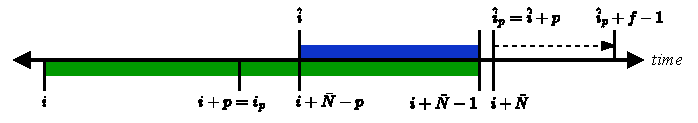
\includegraphics[width=8.4cm]{docs/manuscript/figures/intervals_DeePC.pdf}%[trim={0.0cm 0.0cm 0.0cm 0.0cm},clip,scale=1.0][trim={0.5cm 0.8cm 0.8cm 0.3cm},clip,width=8.4cm]
	\caption{Data ranges used, as shown in a fully adaptive setting (for which $i+\bar{N}=\hat{i}_p$).}
	\label{fig:intervals_DDC}
\end{figure}

Without knowledge of the system matrices $\{A,B,C,D,K\}$ and the initial state $x_\mathrm{ini}$, but given sufficiently informative past input-output data from  intervals $k\in[i,\,i+\bar{N})$ and $k\in[\hat{i},\,\hat{i}_p)$ that may overlap\footnote{Depending on the difference $\hat{i}-i>0$ and the number of samples $\bar{N}$.} and have been collected in closed-loop, the principal goal is to find an unbiased behavioural output predictor to replace the unknown relations \eqref{eq:SS_iter} and \eqref{eq:x_ini}.


\section{Closed-loop Data-enabled Predictive Control}
This section presents the main result of this article, providing contribution~(\ref{contribution:solves_CL_issue}) whereby we develop \ac{CL-DeePC}. An intuitive explanation is first offered before a proof of the underlying main result is provided.

As a solution to the identification bias that arises in closed-loop due to correlation between inputs and noise (a demonstration thereof is deferred to Section~\ref{sec:CL_ID_issue}) it is possible to estimate a step-ahead predictor~\citep{Ljung1996}. A prediction horizon length $f>1$ is of more practical use in receding horizon optimal control settings, to which end step-ahead predictors can be applied sequentially. 

Fig.~\ref{fig:CL-DeePC} and \eqref{eq:CL_DeePC_no_IVs} illustrate how this idea is employed in \ac{CL-DeePC}. A step-ahead predictor can be obtained from \ac{DeePC} (see Fig.~\ref{fig:regular-DeePC} and \eqref{eq:regular_DeePC_no_IVs}) with $f=1$. In \ac{CL-DeePC} the successive columns of $G$ (from left to right) and their corresponding columns on the right-hand side correspond to sequential applications of \ac{DeePC} with $f=1$ to the same matrix of sufficiently persistently exciting past input-output data on the left-hand side as well as time-shifted windows of input-output data on the right-hand side that encode information on successive initial states.\\ 
%
\begin{figure}[b!]
\centering
\begin{tikzpicture}
    % defining constants
    \def\stepSize{0.25}
    \def\Nnum{9}
    \def\fnum{8}
    \def\pnum{4}
    
    % Defining lengths
    \newlength{\onelen}
    \setlength{\onelen}{\stepSize cm}
    \newlength{\BrCl}
    \setlength{\BrCl}{0.075cm}
    \newlength{\BrIn}
    \setlength{\BrIn}{0.15cm}
    \newlength{\plen}
    \setlength{\plen}{1cm}%{\pnum\stepSize cm}
    \newlength{\flen}
    \setlength{\flen}{2cm}%{\fnum*\stepSize cm}
    \newlength{\Nlen}
    \setlength{\Nlen}{2.25cm}%{\Nnum\stepSize cm}%should be 2*p+one
    \newlength{\MatClearance}
    \setlength{\MatClearance}{0.3cm}
    
    % grid lines for guidance
    % \draw[gray,step=0.5] (-0,-3) grid (8,3);

    % ======================= drawing data matrix =======================
    \path (0,-\onelen) coordinate (M1A);
    \path ([xshift=\Nlen]M1A) coordinate (M1B);
    \path ([yshift=2*\plen+2*\onelen]M1B) coordinate (M1C);
    \path ([xshift=-\Nlen]M1C) coordinate (M1D);
    \draw[line width=1.5pt] ([xshift=\BrIn,yshift=-\BrCl]M1A) -- ([xshift=-\BrCl,yshift=-\BrCl]M1A) -- ([xshift=-\BrCl,yshift=\BrCl]M1D) -- ([xshift=\BrIn,yshift=\BrCl]M1D); %left bracket
    \draw[line width=1.5pt] ([xshift=-\BrIn,yshift=-\BrCl]M1B) -- ([xshift=\BrCl,yshift=-\BrCl]M1B) -- ([xshift=\BrCl,yshift=\BrCl]M1C) -- ([xshift=-\BrIn,yshift=\BrCl]M1C); %right bracket
    \draw[line width=1pt] ([yshift=\onelen]M1A) -- ([yshift=\onelen]M1B); % dividing matrix into blocks
    \fill[black, opacity=0.5] (M1A) rectangle (M1C);
    \foreach \x in {0,...,8} { % drawing black dots
    \foreach \y in {-1,...,8} {
      \fill ( {(\x+0.5)*\onelen}, {(\y+0.5)*\onelen} ) circle (1pt);
    }}
    \draw[line width=0.1pt] ([yshift=-\plen-\onelen]M1D) -- ([yshift=-\plen-\onelen]M1C);
    \draw[line width=0.1pt] ([yshift=-\plen]M1D) -- ([yshift=-\plen]M1C);

    % coordinates for diagonals
    \path ([yshift=-\plen]M1D) coordinate (M1stair1A);
    \path ([xshift=\plen]M1D) coordinate (M1stair1I);
    % black diagonals
    % \foreach \i in {0,-1}{
    % \foreach \dy in {1,...,11}{
    % \ifthenelse{\dy<5.5}{
    % % This code will be executed if \dy<9.5
    %     \draw[dash pattern=on 1pt off 2pt, line width=0.1pt] ([xshift= 0.5*\onelen,yshift=\i*(\plen+\onelen)-(\dy+0.5)*\onelen]M1D) -- ([xshift= (\dy+0.5)*\onelen,yshift=\i*(\plen+\onelen)-0.5*\onelen]M1D);
    % }{
    % % This code will be executed if \dy>=10
    %     \ifthenelse{\dy<8.5}{
    %         % This code will be executed if \dy<=12
    %         \draw[dash pattern=on 1pt off 2pt, line width=0.1pt] ([xshift= (\dy-3.5)*\onelen,yshift=\i*(\plen+\onelen)-\plen-\onelen+0.5*\onelen]M1D) -- ([xshift=(\dy-8.5)*\onelen,yshift=\i*(\plen+\onelen)-0.5\onelen]M1C);
    %         }{
    %         % This code will be executed if \dy>=13
    %         \draw[dash pattern=on 1pt off 2pt, line width=0.1pt] ([xshift= (\dy-3.5)*\onelen,yshift=(\i-1)*(\plen+\onelen)+0.5\onelen]M1D) -- ([xshift= -0.5*\onelen,yshift=\i*(\plen+\onelen)-(\dy-7.5)*\onelen]M1C);
    %     }
    % }
    % }}
    
    % ---------------- drawing left brace and matrix ----------------
    \path ([xshift=-0.5\BrIn,yshift=-2\BrCl]M1A) coordinate (Brace1L);
    \path ([xshift=0.5\BrIn,yshift=-2\BrCl]M1B) coordinate (Brace1R);
    \draw[decorate, decoration={calligraphic brace, amplitude=3pt, mirror, aspect=0.75},line width=1pt] (Brace1L) -- (Brace1R);
    \node (mat1) at ($(Brace1L)!0.75!(Brace1R) + (0,-3pt)$) {};
    \node[below] at (mat1.center) {$\begin{bmatrix}
        U_{i,p,N}\\U_{i_p,1,N}\\Y_{i,p,N}\\ \hline Y_{i_p,1,N}
    \end{bmatrix}$};
    % brace to the left
    % \path ([xshift=-0.75cm-0.05cm,yshift=-4pt]mat1.center) coordinate (Brace1T);
    % \path ([yshift=-1.73cm]Brace1T) coordinate (Brace1B);
    % \draw[pen colour=gray!60,decorate, decoration={calligraphic brace, amplitude=3pt, mirror, aspect=0.2},line width=0.75pt] (Brace1T) -- (Brace1B);
    % % Zp
    % \node (Zp) at ($(Brace1T)!0.2!(Brace1B) + (-3pt,-0.8pt)$) {};
    % \node[left,text=gray!100,align=center] at ([xshift=0.5mm,yshift=-0.18cm]Zp.center) {\scriptsize{\shortstack{$=$\\$\Phi_{i,1,N}$}}};
  
    % ======================= drawing G =======================
    % useful coordinates
    \path ([xshift=\MatClearance,yshift=\onelen]M1B) coordinate (M2A);
    \path ([xshift=\flen]M2A) coordinate (M2B);
    \path ([yshift=\Nlen]M2B) coordinate (M2C);
    \path ([xshift=-\flen]M2C) coordinate (M2D);

    % brackets
    \draw[line width=1.5pt] ([xshift=\BrIn,yshift=-\BrCl]M2A) -- ([xshift=-\BrCl,yshift=-\BrCl]M2A) -- ([xshift=-\BrCl,yshift=\BrCl]M2D) -- ([xshift=\BrIn,yshift=\BrCl]M2D); %left bracket
    \draw[line width=1.5pt] ([xshift=-\BrIn,yshift=-\BrCl]M2B) -- ([xshift=\BrCl,yshift=-\BrCl]M2B) -- ([xshift=\BrCl,yshift=\BrCl]M2C) -- ([xshift=-\BrIn,yshift=\BrCl]M2C); %right bracket
    
    % red fill
    \fill[red!50,opacity=0.5] (M2A) rectangle (M2C);

    % drawing red dots
    \foreach \x in {0,...,7} {
    \foreach \y in {0,...,8} {
      \fill[red] ([xshift=(\x+0.5)*\onelen,yshift=(\y+0.5)*\onelen]M2A) circle (1pt);%{(\x+0.5)*\onelen+\Nlen+0.5cm}, {(\y+0.5)*\onelen}
    }}

    % dividers
    \foreach \x in {1,...,7}{\draw[line width=0.1pt] ([xshift=\x*\onelen]M2A) -- ([xshift=\x*\onelen]M2D);}

    % drawing middle brace and matrix
    \coordinate (Brace2L) at ([xshift=-0.5\BrIn]M2A |- Brace1L);
    \coordinate (Brace2R) at ([xshift=0.5\BrIn]M2B |- Brace1L);
    \draw[decorate, decoration={calligraphic brace, amplitude=3pt, mirror, aspect=0.5},line width=1pt] (Brace2L) -- (Brace2R);
    \node (mat1) at ($(Brace2L)!0.5!(Brace2R) + (0,-3pt)$) {};
    \node[below] at ([yshift=-0.75cm]mat1.center) {$\underbrace{
    \begin{bmatrix}
        g_1 & g_2 & \cdots & g_f
    \end{bmatrix}}_{= G}$};
    
    % ======================= drawing equal sign ======================= 
    \path ([xshift=\MatClearance*3/4,yshift=\Nlen/2-0.1cm]M2B) coordinate (EqA);
    \path ([xshift=0.4cm]EqA) coordinate (EqB);
    \path ([yshift=0.2cm]EqB) coordinate (EqC);
    \path ([xshift=-0.4cm]EqC) coordinate (EqD);
    \draw[line width = 1.5 pt] (EqA) -- (EqB);
    \draw[line width = 1.5 pt] (EqD) -- (EqC);

    % ---------------- equation sign below ----------------
    \node[below] at ([xshift=5.65\onelen,yshift=-1.05cm]mat1.center) {$=$};

    % ======================= drawing RHS =======================
    % inside of matrix
    \path ([xshift=\MatClearance*3/4,yshift=-\Nlen/2+0.1cm-\onelen]EqB) coordinate (M3A);
    \path ([xshift=\flen]M3A) coordinate (M3B);
    \path ([yshift=2*\plen+2*\onelen]M3B) coordinate (M3C);
    \path ([xshift=-\flen]M3C) coordinate (M3D);
    % top left black triangle
    \path ([yshift=-\plen-\onelen/2]M3D) coordinate (t1A);
    \path ([xshift=\plen+\onelen/2]M3D) coordinate (t1B);
    % top red trapezoid
    \path ([yshift=-\onelen/2]t1A) coordinate (t2A);
    \path ([xshift=\flen]t2A) coordinate (t2B);
    % bottom black triangle
    \path ([yshift=-\plen-\onelen/2]t2A) coordinate (t3A);
    \path ([xshift=\plen+\onelen/2]t2A) coordinate (t3B);
    % bottom red trapezoid
    \path ([yshift=-\onelen/2]t3A) coordinate (t4A);

    % top 'staircase' coordinates
    \path ([yshift=-\plen]M3D) coordinate (stair1A);
    \path ([xshift=\onelen]stair1A) coordinate (stair1B);
    \path ([yshift=\onelen]stair1B) coordinate (stair1C);
    \path ([xshift=\onelen]stair1C) coordinate (stair1D);
    \path ([yshift=\onelen]stair1D) coordinate (stair1E);
    \path ([xshift=\onelen]stair1E) coordinate (stair1F);
    \path ([yshift=\onelen]stair1F) coordinate (stair1G);
    \path ([xshift=\onelen]stair1G) coordinate (stair1H);
    \path ([yshift=\onelen]stair1H) coordinate (stair1I);

    % bottom 'staircase' coordinates
    \path ([yshift=-\onelen]stair1A) coordinate (stair2J);
    \path ([yshift=-\plen]stair2J) coordinate (stair2A);
    \path ([xshift=\onelen]stair2A) coordinate (stair2B);
    \path ([yshift=\onelen]stair2B) coordinate (stair2C);
    \path ([xshift=\onelen]stair2C) coordinate (stair2D);
    \path ([yshift=\onelen]stair2D) coordinate (stair2E);
    \path ([xshift=\onelen]stair2E) coordinate (stair2F);
    \path ([yshift=\onelen]stair2F) coordinate (stair2G);
    \path ([xshift=\onelen]stair2G) coordinate (stair2H);
    \path ([yshift=\onelen]stair2H) coordinate (stair2I);
    
    % fill figures
    % \fill[black, opacity=0.5]  (t1A) -- (t1B) -- (M3D) -- cycle;% top black
    % \fill[red!50, opacity=0.5] (t2A) -- (t2B) -- (M3C) -- (t1B) -- (t1A) -- cycle;% top red
    % \fill[black, opacity=0.5]  (t3A) -- (t3B) -- (t2A) -- cycle;% bottom black
    % \fill[red!50, opacity=0.5] (t4A) -- (M3B) -- (t2B) -- (t3B) -- (t3A) -- cycle; % bottom red
    \fill[black,opacity=0.5]  (M3D) -- (stair1A) -- (stair1B) -- (stair1C) -- (stair1D) -- (stair1E) -- (stair1F) -- (stair1G) -- (stair1H) -- (stair1I) -- cycle;
    \fill[red!50,opacity=0.5] ([xshift=\flen-\onelen]stair1B) -- (stair1B) -- (stair1C) -- (stair1D) -- (stair1E) -- (stair1F) -- (stair1G) -- (stair1H) -- (stair1I) -- (M3C) -- cycle;
    \fill[black,opacity=0.5]  (stair2J) -- (stair2A) -- (stair2B) -- (stair2C) -- (stair2D) -- (stair2E) -- (stair2F) -- (stair2G) -- (stair2H) -- (stair2I) -- cycle;
    \fill[red!50,opacity=0.5] ([xshift=\flen-\onelen]stair2B) -- (stair2B) -- (stair2C) -- (stair2D) -- (stair2E) -- (stair2F) -- (stair2G) -- (stair2H) -- (stair2I) -- ([yshift=-\plen-\onelen]M3C) -- cycle;
    
    % draw brackets
    \draw[line width=1.5pt] ([xshift=\BrIn,yshift=-\BrCl]M3A) -- ([xshift=-\BrCl,yshift=-\BrCl]M3A) -- ([xshift=-\BrCl,yshift=\BrCl]M3D) -- ([xshift=\BrIn,yshift=\BrCl]M3D); %left bracket
    \draw[line width=1.5pt] ([xshift=-\BrIn,yshift=-\BrCl]M3B) -- ([xshift=\BrCl,yshift=-\BrCl]M3B) -- ([xshift=\BrCl,yshift=\BrCl]M3C) -- ([xshift=-\BrIn,yshift=\BrCl]M3C); %right bracket
    
    % U_{i,p,N}
    \path ([xshift=0.5*\onelen,yshift=-\plen+0.5*\onelen]M3D) coordinate (tlbA);
    \foreach \x in {0,...,7}{
    \foreach \y in {0,...,3}{
        \ifthenelse{{\y>\x}\OR{\y=\x}}{%
        % \fill[black, opacity=0.5] ([xshift={(\x-0.5)*\onelen},yshift={(\y-0.5)*\onelen}]tlbA) rectangle ([xshift={(\x+0.5)*\onelen},yshift={(\y+0.5)*\onelen}]tlbA);
        \fill[black] ([xshift={\x*\onelen},yshift={\y*\onelen}]tlbA) circle (1pt);
        }{%
        % \fill[red!50,opacity=0.5] ([xshift={(\x-0.5)*\onelen},yshift={(\y-0.5)*\onelen}]tlbA) rectangle ([xshift={(\x+0.5)*\onelen},yshift={(\y+0.5)*\onelen}]tlbA);%<do this if false>
        \fill[red] ([xshift={\x*\onelen},yshift={(\y*\onelen}]tlbA) circle (1pt);
        }%
    }}
    
    % U_{i_p,1,N}
    \path ([yshift=-\onelen]tlbA) coordinate (tlbB);
    \fill[red!50,opacity=0.5] (stair1A) rectangle ([xshift=\flen,yshift=-\onelen]stair1A);
    \foreach \x in {0,...,7}{\fill[red] ([xshift=\x*\onelen]tlbB) circle (1pt);}
    
    % Y_{i,p,N}
    \path ([yshift=-\plen]tlbB) coordinate (tlbC);
    \foreach \x in {0,...,7}{
    \foreach \y in {0,...,3}{
        \ifthenelse{{\y>\x}\OR{\y=\x}}{%
        \fill[black] ([xshift={\x*\onelen},yshift={\y*\onelen}]tlbC) circle (1pt);%<do this if true>
        }{%
        \fill[red] ([xshift={\x*\onelen},yshift={(\y*\onelen}]tlbC) circle (1pt);%<do this if false>
        }%
    }}

    % Y_{i_p,1,N}
    \path ([yshift=-\onelen]tlbC) coordinate (tlbD);
    \fill[red!50,opacity=0.5] (stair2A) rectangle ([xshift=\flen,yshift=-\onelen]stair2A);
    \foreach \x in {0,...,7}{\fill[red] ([xshift=\x*\onelen]tlbD) circle (1pt);}

    \foreach \dy in {0,-\plen-\onelen}{%
    % black diagonals
    \draw[dash pattern=on 1pt off 2pt, line width=0.1pt] ([xshift= 1/2*\onelen,yshift=\dy+5/2*\onelen]stair1A) -- ([xshift=-5/2*\onelen,yshift=\dy-1/2*\onelen]stair1I);
    \draw[dash pattern=on 1pt off 2pt, line width=0.1pt] ([xshift= 1/2*\onelen,yshift=\dy+3/2*\onelen]stair1A) -- ([xshift=-3/2*\onelen,yshift=\dy-1/2*\onelen]stair1I);
    \draw[dash pattern=on 1pt off 2pt, line width=0.1pt] ([xshift= 1/2*\onelen,yshift=\dy+1/2*\onelen]stair1A) -- ([xshift=-1/2*\onelen,yshift=\dy-1/2*\onelen]stair1I);
    % red diagonals
    \draw[red,dash pattern=on 1pt off 2pt, line width=0.1pt] ([xshift= 1/2*\onelen,yshift=\dy-1/2*\onelen]stair1A) -- ([xshift=1/2*\onelen,yshift=\dy-1/2*\onelen]stair1I);
    \draw[red,dash pattern=on 1pt off 2pt, line width=0.1pt] ([xshift= 3/2*\onelen,yshift=\dy-1/2*\onelen]stair1A) -- ([xshift=3/2*\onelen,yshift=\dy-1/2*\onelen]stair1I);
    \draw[red,dash pattern=on 1pt off 2pt, line width=0.1pt] ([xshift= 5/2*\onelen,yshift=\dy-1/2*\onelen]stair1A) -- ([xshift=5/2*\onelen,yshift=\dy-1/2*\onelen]stair1I);
    \draw[red,dash pattern=on 1pt off 2pt, line width=0.1pt] ([xshift= 7/2*\onelen,yshift=\dy-1/2*\onelen]stair1A) -- ([xshift=7/2*\onelen,yshift=\dy-1/2*\onelen]stair1I);
    \draw[red,dash pattern=on 1pt off 2pt, line width=0.1pt] ([xshift= 9/2*\onelen,yshift=\dy-1/2*\onelen]stair1A) -- ([xshift=7/2*\onelen,yshift=\dy-3/2*\onelen]stair1I);
    \draw[red,dash pattern=on 1pt off 2pt, line width=0.1pt] ([xshift=11/2*\onelen,yshift=\dy-1/2*\onelen]stair1A) -- ([xshift=7/2*\onelen,yshift=\dy-5/2*\onelen]stair1I);
    \draw[red,dash pattern=on 1pt off 2pt, line width=0.1pt] ([xshift=13/2*\onelen,yshift=\dy-1/2*\onelen]stair1A) -- ([xshift=7/2*\onelen,yshift=\dy-7/2*\onelen]stair1I);
    }
    
    % draw dividers
    \draw[line width=0.1pt] ([yshift=-\plen-\onelen]M3D) -- ([yshift=-\plen-\onelen]M3C);
    \draw[line width=0.1pt] ([yshift=-\plen]M3D) -- ([yshift=-\plen]M3C);
    \draw[line width=1pt] ([yshift=\onelen]M3A) -- ([yshift=\onelen]M3B);

    % ---------------- drawing right brace and matrix ----------------
    % brace below matrix
    \path ([xshift=-0.5\BrIn,yshift=-2\BrCl]M3A) coordinate (Brace3L);
    \path ([xshift=0.5\BrIn,yshift=-2\BrCl]M3B) coordinate (Brace3R);
    \draw[decorate, decoration={calligraphic brace, amplitude=3pt, mirror, aspect=0.25},line width=1pt] (Brace3L) -- (Brace3R);
    % matrix below brace
    \node (mat3) at ($(Brace3L)!0.25!(Brace3R) + (0,-3pt)$) {};
    \node[below] at (mat3.center) {$\begin{bmatrix}
        U_{\hat{i},p,f}\\U_{\hat{i}_p,1,f}\\Y_{\hat{i},p,f}\\ \hline \widehat{Y}_{\hat{i}_p,1,f}
    \end{bmatrix}$};
    % tag & label (on RHS of column)
    \node[below] at ([xshift=2.13cm,yshift=-0.9cm]mat3.center) {$\refstepcounter{equation}(\theequation)\label{eq:CL_DeePC_no_IVs}$};
    % brace to the right
    % \path ([xshift=0.7cm+0.05cm]mat3.center |- Brace1T) coordinate (Brace3T);%([xshift=0.7cm,yshift=-4pt]mat3.center) coordinate (Brace3T);
    % \path (Brace3T |- Brace1B) coordinate (Brace3B);
    % \draw[pen colour=gray!60,decorate, decoration={calligraphic brace, amplitude=3pt, aspect=0.2},line width=0.75pt] (Brace3T) -- (Brace3B);
    % % Zf
    % \node (Zf) at ($(Brace3T)!0.2!(Brace3B) + (3pt,-1.5pt)$) {};
    % \node[right,text=gray!100] at ([yshift=-0.18cm]Zf.center) {\scriptsize{\shortstack{$=$\\$\Phi_{\hat{i},1,f}$}}};
    
    % ======================= length indicators ======================= 
    \draw[|-|] ([yshift=\onelen]M1D) -- node[above] {\scriptsize$N$} ([yshift=\onelen]M1C);
    \draw[|-|] ([yshift=\onelen]M2D) -- node[above] {\scriptsize$f$} ([yshift=\onelen]M2C);
    \draw[|-|] ([yshift=\onelen]M3D) -- node[above] {\scriptsize$f$} ([yshift=\onelen]M3C);
    \draw[|-|] ([xshift=\onelen]M3C) -- node[right] {\scriptsize$pr$} ([xshift=\onelen,yshift=\onelen]t2B);
    \draw[|-|] ([xshift=\onelen,yshift=\onelen]t2B) -- node[right] {\scriptsize$r$} ([xshift=\onelen]t2B);
    \draw[|-|] ([xshift=\onelen]t2B) -- node[right] {\scriptsize$pl$} ([xshift=\onelen,yshift=\onelen]M3B);
    \draw[|-|] ([xshift=\onelen,yshift=\onelen]M3B) -- node[right] {\scriptsize$l$} ([xshift=\onelen]M3B);
\end{tikzpicture}
\caption{Visualization of known (black) and unknown (red) variables in \ac{CL-DeePC} without \ac{IVs}. Each dot represents an input $u_k\in\mathbb{R}^r$, output $y_k\in\mathbb{R}^l$, or element of the matrix $G$. \ac{CL-DeePC} involves $f$ sequential applications of a step-ahead predictor obtained from regular \ac{DeePC} with $f=1$ (see also Fig.~\ref{fig:regular-DeePC}), resulting in the dashed block-anti diagonals with the same $u_k$ or $y_k$ on the right hand side.}
\label{fig:CL-DeePC}
\end{figure}
\begin{figure}[b!]
\centering
\begin{tikzpicture}
    % defining constants
    \def\stepSize{0.25}
    \def\Nnum{9}
    \def\fnum{8}
    \def\pnum{4}
    
    % Defining lengths
    % \newlength{\onelen}
    \setlength{\onelen}{\stepSize cm}
    % \newlength{\BrCl}
    \setlength{\BrCl}{0.075cm}
    % \newlength{\BrIn}
    \setlength{\BrIn}{0.15cm}
    % \newlength{\plen}
    \setlength{\plen}{1cm}%{\pnum\stepSize cm}
    % \newlength{\flen}
    \setlength{\flen}{2cm}%{\fnum*\stepSize cm}
    % \newlength{\Nlen}
    \setlength{\Nlen}{2.25cm}%{\Nnum\stepSize cm}%should be 2*p+one
    % \newlength{\MatClearance}
    \setlength{\MatClearance}{0.3cm}
    
    % grid lines for guidance
    % \draw[gray,step=0.5] (-0,-7) grid (8,3);

    % ======================= drawing data matrix =======================
    \path (0,2\plen+\onelen) coordinate (M1D);
    \path ([yshift=-2\plen-2\flen]M1D) coordinate (M1A);
    \path ([xshift=\Nlen]M1A) coordinate (M1B);
    \path ([yshift=2*\plen+2*\flen]M1B) coordinate (M1C);
    \draw[line width=1.5pt] ([xshift=\BrIn,yshift=-\BrCl]M1A) -- ([xshift=-\BrCl,yshift=-\BrCl]M1A) -- ([xshift=-\BrCl,yshift=\BrCl]M1D) -- ([xshift=\BrIn,yshift=\BrCl]M1D); %left bracket
    \draw[line width=1.5pt] ([xshift=-\BrIn,yshift=-\BrCl]M1B) -- ([xshift=\BrCl,yshift=-\BrCl]M1B) -- ([xshift=\BrCl,yshift=\BrCl]M1C) -- ([xshift=-\BrIn,yshift=\BrCl]M1C); %right bracket
    \draw[line width=1pt] ([yshift=\flen]M1A) -- ([yshift=\flen]M1B); % dividing matrix into blocks
    \fill[black, opacity=0.5] (M1A) rectangle (M1C);
    \foreach \x in {0,...,8} { % drawing black dots
    \foreach \y in {-15,...,8} {
      \fill ( {(\x+0.5)*\onelen}, {(\y+0.5)*\onelen} ) circle (1pt);
    }}
    \draw[line width=0.1pt] ([yshift=-\plen-\flen]M1D) -- ([yshift=-\plen-\flen]M1C);
    \draw[line width=0.1pt] ([yshift=-\plen]M1D) -- ([yshift=-\plen]M1C);

    % coordinates for diagonals
    \path ([yshift=-\plen]M1D) coordinate (M1stair1A);
    \path ([xshift=\Nlen]M1D) coordinate (M1stair1I);
    % black diagonals
    % \foreach \i in {0,-1}{
    % \foreach \dy in {1,...,18}{
    % \ifthenelse{\dy<9.5}{
    % % This code will be executed if \dy<9.5
    %     \draw[dash pattern=on 1pt off 2pt, line width=0.1pt] ([xshift= 0.5*\onelen,yshift=\i*(\plen+\flen)-(\dy+0.5)*\onelen]M1D) -- ([xshift= (\dy+0.5)*\onelen,yshift=\i*(\plen+\flen)-0.5*\onelen]M1D);
    % }{
    % % This code will be executed if \dy>=10
    %     \ifthenelse{\dy<12.5}{
    %         % This code will be executed if \dy<=12
    %         \draw[dash pattern=on 1pt off 2pt, line width=0.1pt] ([xshift= 0.5*\onelen,yshift=\i*(\plen+\flen)-(\dy+0.5)*\onelen]M1D) -- ([xshift= -0.5*\onelen,yshift=\i*(\plen+\flen)-(\dy-7.5)*\onelen]M1C);
    %         }{
    %         % This code will be executed if \dy>=13
    %         \draw[dash pattern=on 1pt off 2pt, line width=0.1pt] ([xshift= (\dy-10.5)*\onelen,yshift=\i*(\plen+\flen)-\plen-\flen+0.5*\onelen]M1D) -- ([xshift= -0.5*\onelen,yshift=\i*(\plen+\flen)-(\dy-7.5)*\onelen]M1C);
    %     }
    % }
    % }}
    
    % ---------------- drawing left brace and matrix ----------------
    \path ([xshift=-0.5\BrIn,yshift=-2\BrCl]M1A) coordinate (Brace1L);
    \path ([xshift=0.5\BrIn,yshift=-2\BrCl]M1B) coordinate (Brace1R);
    \draw[decorate, decoration={calligraphic brace, amplitude=3pt, mirror, aspect=0.75},line width=1pt] (Brace1L) -- (Brace1R);
    \node (mat1) at ($(Brace1L)!0.75!(Brace1R) + (0,-3pt)$) {};
    \node[below] at (mat1.center) {$\begin{bmatrix}
        U_{i,p,N}\\U_{i_p,f,N}\\Y_{i,p,N}\\ \hline Y_{i_p,f,N}
    \end{bmatrix}$};
    % brace to the left
    % \path ([xshift=-0.75cm-0.05cm,yshift=-4pt]mat1.center) coordinate (Brace1T);
    % \path ([yshift=-1.73cm]Brace1T) coordinate (Brace1B);
    % \draw[pen colour=gray!60,decorate, decoration={calligraphic brace, amplitude=3pt, mirror, aspect=0.2},line width=0.75pt] (Brace1T) -- (Brace1B);
    % % Zp
    % \node (Zp) at ($(Brace1T)!0.2!(Brace1B) + (-3pt,-0.8pt)$) {};
    % \node[left,text=gray!100,align=center] at ([xshift=0.5mm,yshift=-0.18cm]Zp.center) {\scriptsize{\shortstack{$=$\\$\Phi_{i,f,N}$}}};
  
    % ======================= drawing G =======================
    % useful coordinates
    \path ([xshift=\MatClearance,yshift=-0.5\Nlen-\plen-\flen]M1C) coordinate (M2A);
    \path ([xshift=\onelen]M2A) coordinate (M2B);
    \path ([yshift=\Nlen]M2B) coordinate (M2C);
    \path ([xshift=-\onelen]M2C) coordinate (M2D);

    % brackets
    \draw[line width=1.5pt] ([xshift=0.5\BrIn,yshift=-\BrCl]M2A) -- ([xshift=-\BrCl,yshift=-\BrCl]M2A) -- ([xshift=-\BrCl,yshift=\BrCl]M2D) -- ([xshift=0.5\BrIn,yshift=\BrCl]M2D); %left bracket
    \draw[line width=1.5pt] ([xshift=-0.5\BrIn,yshift=-\BrCl]M2B) -- ([xshift=\BrCl,yshift=-\BrCl]M2B) -- ([xshift=\BrCl,yshift=\BrCl]M2C) -- ([xshift=-0.5\BrIn,yshift=\BrCl]M2C); %right bracket
    
    % red fill
    \fill[red!50,opacity=0.5] (M2A) rectangle (M2C);

    % drawing red dots
    \foreach \x in {0} {
    \foreach \y in {0,...,8} {
      \fill[red] ([xshift=(\x+0.5)*\onelen,yshift=(\y+0.5)*\onelen]M2A) circle (1pt);
    }}

    % drawing middle brace and matrix
    \coordinate (Brace2L) at ([xshift=-0.5\BrIn]M2A |- Brace1L);
    \coordinate (Brace2R) at ([xshift=0.5\BrIn]M2B |- Brace1L);
    \draw[decorate, decoration={calligraphic brace, amplitude=3pt, mirror, aspect=0.5},line width=1pt] (Brace2L) -- (Brace2R);
    \node (mat1) at ($(Brace2L)!0.5!(Brace2R) + (0,-3pt)$) {};
    \node[below] at ([yshift=-1.05cm]mat1.center) {$g$};
    
    % ======================= drawing equal sign ======================= 
    \path ([xshift=\MatClearance*3/4,yshift=\Nlen/2-0.1cm]M2B) coordinate (EqA);
    \path ([xshift=0.4cm]EqA) coordinate (EqB);
    \path ([yshift=0.2cm]EqB) coordinate (EqC);
    \path ([xshift=-0.4cm]EqC) coordinate (EqD);
    \draw[line width = 1.5 pt] (EqA) -- (EqB);
    \draw[line width = 1.5 pt] (EqD) -- (EqC);

    % ---------------- equation sign below ----------------
    \node[below] at ([xshift=2\onelen,yshift=-1.05cm]mat1.center) {$=$};

    % ======================= drawing RHS =======================
    % inside of matrix
    \path ([xshift=0.75\MatClearance]EqB |- M1A) coordinate (M3A);
    \path ([xshift=\onelen]M3A) coordinate (M3B);
    \path ([yshift=2\plen+2\flen]M3B) coordinate (M3C);
    \path ([xshift=-\onelen]M3C) coordinate (M3D);
    
    % fill figures
    \fill[black,opacity=0.5]  (M3D) -- ([yshift=-\plen]M3D) -- ([yshift=-\plen]M3C) -- (M3C) -- cycle;
    \fill[red!50,opacity=0.5] ([yshift=-\plen]M3D) -- ([yshift=-\plen-\flen]M3D) -- ([yshift=-\plen-\flen]M3C) -- ([yshift=-\plen]M3C) -- cycle;
    \fill[black,opacity=0.5] ([yshift=\flen]M3A) -- ([yshift=\flen]M3B) -- ([yshift=\flen+\plen]M3B) -- ([yshift=\flen+\plen]M3A) -- cycle;
    \fill[red!50,opacity=0.5]  (M3A) -- (M3B) -- ([yshift=\flen]M3B) -- ([yshift=\flen]M3A) -- cycle;
    
    % draw brackets
    \draw[line width=1.5pt] ([xshift=0.5\BrIn,yshift=-\BrCl]M3A) -- ([xshift=-\BrCl,yshift=-\BrCl]M3A) -- ([xshift=-\BrCl,yshift=\BrCl]M3D) -- ([xshift=0.5\BrIn,yshift=\BrCl]M3D); %left bracket
    \draw[line width=1.5pt] ([xshift=-0.5\BrIn,yshift=-\BrCl]M3B) -- ([xshift=\BrCl,yshift=-\BrCl]M3B) -- ([xshift=\BrCl,yshift=\BrCl]M3C) -- ([xshift=-0.5\BrIn,yshift=\BrCl]M3C); %right bracket
    
    % U_{i,p,1}
    \foreach \dy in {0,...,-3}{
        \fill[black] ([xshift=0.5\onelen,yshift=(\dy-0.5)*\onelen]M3D) circle (1pt);
    }

    % U_{i_p,f,1}
    \foreach \dy in {-4,...,-11}{
        \fill[red] ([xshift=0.5\onelen,yshift=(\dy-0.5)*\onelen]M3D) circle (1pt);
    }
    
    % Y_{i,p,1}
    \foreach \dy in {0,...,-3}{
        \fill[black] ([xshift=0.5\onelen,yshift=(\dy-0.5)*\onelen-\plen-\flen]M3D) circle (1pt);
    }

    % Y_{i_p,f,1}
    \foreach \dy in {-4,...,-11}{
        \fill[red] ([xshift=0.5\onelen,yshift=(\dy-0.5)*\onelen-\plen-\flen]M3D) circle (1pt);
    }

    % draw dividers
    \draw[line width=0.1pt] ([yshift=-\plen]M3D) -- ([yshift=-\plen]M3C);
    \draw[line width=0.1pt] ([yshift=-\plen-\flen]M3D) -- ([yshift=-\plen-\flen]M3C);
    \draw[line width=1pt] ([yshift=\flen]M3A) -- ([yshift=\flen]M3B);

    % ---------------- drawing right brace and matrix ----------------
    % brace below matrix
    \path ([xshift=-0.5\BrIn,yshift=-2\BrCl]M3A) coordinate (Brace3L);
    \path ([xshift=0.5\BrIn,yshift=-2\BrCl]M3B) coordinate (Brace3R);
    \draw[decorate, decoration={calligraphic brace, amplitude=3pt, mirror, aspect=0.5},line width=1pt] (Brace3L) -- (Brace3R);
    % matrix below brace
    \node (mat3) at ($(Brace3L)!0.5!(Brace3R) + (0,-3pt)$) {};
    \node[below] at ([xshift=0.35cm]mat3.center) {$\begin{bmatrix}
        U_{\hat{i},p,1}\\U_{\hat{i}_p,f,1}\\Y_{\hat{i},p,1}\\ \hline \widehat{Y}_{\hat{i}_p,f,1}
    \end{bmatrix}$};
    % tag & label (on RHS of column)
    \node[below left] at (8.35cm,-5cm) {$\refstepcounter{equation}(\theequation)\label{eq:regular_DeePC_no_IVs}$};
    % brace to the right
    % \path ([xshift=1.1cm]mat3.center |- Brace1T) coordinate (Brace3T);%([xshift=0.7cm,yshift=-4pt]mat3.center) coordinate (Brace3T);
    % \path (Brace3T |- Brace1B) coordinate (Brace3B);
    % \draw[pen colour=gray!60,decorate, decoration={calligraphic brace, amplitude=3pt, aspect=0.2},line width=0.75pt] (Brace3T) -- (Brace3B);
    % % Zf
    % \node (Zf) at ($(Brace3T)!0.2!(Brace3B) + (3pt,-1.5pt)$) {};
    % \node[right,text=gray!100] at ([yshift=-0.18cm]Zf.center) {\scriptsize{\shortstack{$=$\\$\Phi_{\hat{i},f,1}$}}};
    
    % ======================= length indicators ======================= 
    \draw[|-|] ([yshift=\onelen]M1D) -- node[above] {\scriptsize$N$} ([yshift=\onelen]M1C);
    \draw[|-|] ([xshift=\onelen]M3C) -- node[right] {\scriptsize$pr$} ([xshift=\onelen,yshift=-\plen]M3C);
    \draw[|-|] ([xshift=\onelen,yshift=-\plen]M3C) -- node[right] {\scriptsize$fr$} ([xshift=\onelen,yshift=-\plen-\flen]M3C);
    \draw[|-|] ([xshift=\onelen,yshift=-\plen-\flen]M3C) -- node[right] {\scriptsize$pl$} ([xshift=\onelen,yshift=\flen]M3B);
    \draw[|-|] ([xshift=\onelen,yshift=\flen]M3B) -- node[right] {\scriptsize$fl$} ([xshift=\onelen]M3B);
\end{tikzpicture}
\caption{Visualization of known (black) and unknown (red) variables in \ac{DeePC} without \ac{IVs}. Each dot represents an input $u_k\in\mathbb{R}^r$, output $y_k\in\mathbb{R}^l$, or element of the matrix $G$. A multi-step ahead predictor of prediction length $f$ is formed directly by taking a linear combination of past input and output data.\\\vspace{0.75mm}}
\label{fig:regular-DeePC}
\end{figure}
%
\setcounter{thm}{0}
\begin{thm}\label{theorem:main_result}
    Consider the minimal discrete non-deterministic \ac{LTI} system given by~\eqref{eqn:SS_innovation} to generate input-output data in closed-loop by means of a causal controller without direct feedthrough, and data matrices $\overline{\Phi}_{\hat{i},1,f}$ and $\Phi_{i,1,N}$ as in \eqref{eq:Phi_def}. %If $\Phi_{i,1,N}$ is both square and invertible %
    %
    If the joint input and noise sequences are sufficiently persistently exciting such that $\left[X_{i,1,N}^\top \; U_{i,p,N}^\top \; U_{i_p,1,N}^\top \; E_{i,p,N}^\top\right]^\top$ is full row rank %
    % ------------------------------------------------------
    %% ----------------- old version below -----------------
    %If the input sequence $\{u_k\}_{k=i}^{i+\bar{N}-1}$ of length $\bar{N}=p+s+N-1$ %, with $N\geq(p+s+n)(r+l)+n$ and $p\geq\ell$\todo{don't forget},
    % is persistently exciting of order $p+s+n$, and has sample correlations such that%
    % \begin{alignat}{2}%see also https://www.cis.upenn.edu/~jean/schur-comp.pdf
    % % \widehat{\Sigma}_{u,u} &> 0,\label{eq:PE_corU}\\
    % &\widehat{\Sigma}_{\mathrm{ee}} - \widehat{\Sigma}_{\mathrm{ue}^\top} \widehat{\Sigma}_{\mathrm{uu}}\inv \widehat{\Sigma}_{\mathrm{ue}}\succ0,\span\span\label{eq:PE_corUE2}\\
    % &&\text{with}\quad\widehat{\Sigma}_{\mathrm{ee}}&=E_{i,p+s+n,N-n}E_{i,p+s+n,N-n}^\top,\notag\\
    % &&\widehat{\Sigma}_{\mathrm{ue}}&=U_{i,p+s+n,N-n}E_{i,p+s+n,N-n}^\top,\notag\\
    % &&\widehat{\Sigma}_{\mathrm{uu}}&=U_{i,p+s+n,N-n}U_{i,p+s+n,N-n}^\top,\notag
    % \end{alignat}
    % ------------------------------------------------------
    then \\
    $\mathrm{(i)}$ $\exists G\in\mathbb{R}^{N\times f}$ such that
    \begin{align}\tag{\ref{eq:CL_DeePC_no_IVs}}%\label{eq:Theorem1}
        \begin{bmatrix}
            \Phi_{i,1,N}\\
            Y_{i_p,1,N}
        \end{bmatrix}G =
        \begin{bmatrix}
            \overline{\Phi}_{\hat{i},1,f}\\
            \widehat{Y}_{\hat{i}_p,1,f}
        \end{bmatrix},
    \end{align}
    $\mathrm{(ii)}$ and with $\widehat{Y}_{\hat{i}_p,1,f}$ as an asymptotically unbiased predictor %with respect to both past and future noise 
    as $p\rightarrow\infty$.
\end{thm}

% ---------------- Proof of (i) ----------------
\noindent\textbf{Proof of $(\mathrm{i})$:} Equation \eqref{eq:CL_DeePC_no_IVs} specifies the output predictor as $\widehat{Y}_{\hat{i}_p,1,f}=\widehat{Y}_{\hat{i}_p,1,f}G$, for which $G$ is determined by\footnote{Although $\overline{\Phi}_{\hat{i},1,f}$ itself contains future output predictions, as shown by \figref{fig:CL-DeePC}, this reliance is strictly causal.} $\Phi_{i,1,N}G=\overline{\Phi}_{\hat{i},1,f}$. There exists at least one solution to this latter equation if $\Phi_{i,1,N}$ is full row rank. Decomposing $\Phi_{i,1,N}$ into its dependencies begets
\begin{align}\label{eq:Phi_isN}
    \mkern-8mu\Phi_{i,1,N}=\mkern-1mu\begin{bmatrix}
        U_{i,p,N}\\
        U_{i_p,1,N}\\
        Y_{i,p,N}
    \end{bmatrix}\mkern-1mu=\mkern-1mu
    \underbrace{\begin{bmatrix}
        0        & I_{pr} & 0      & 0\\
        0        & 0      & I_{r} & 0\\
        \Gamma_p & \mathcal{T}_p^\mathrm{u} & 0 & \mathcal{H}_p
    \end{bmatrix}}\mkern-3mu\begin{bmatrix}
        X_{i,1,N}\\
        U_{i,p,N}\\
        U_{i_p,1,N}\\
        E_{i,p,N}
    \end{bmatrix}\mkern-1mu,
\end{align}
in which the matrix on the right hand side is assumed to be full row rank, and the underbraced matrix is also full row rank. Since both of these matrices are full row rank, so is its product $\Phi_{i,1,N}$, meaning that there exists at least one $G$ that satisfies \eqref{eq:CL_DeePC_no_IVs}. $\hfill\qed$

\noindent\textbf{Remark 1:} For the matrix on the right hand side of \eqref{eq:Phi_isN} to be guaranteed to be of full row rank a necessary condition is that $N\geq n+(p+1)r+pl$.

\noindent\textbf{Remark 2:} The full row rank matrix $\Phi_{i,1,N}\in\mathbb{R}^{((p+1)r+pl)\times N}$ has more columns than rows, meaning that in fact there are an infinite number of possibilities for $G$ that satisfy \eqref{eq:CL_DeePC_no_IVs}. These possibilities are given by
\begin{align}\label{eq:G_sols}
    G = \Phi_{i,1,N}^\dagger\overline{\Phi}_{\hat{i},1,f} + \Pi_{\Phi_{i,1,N}}^\bot W,
\end{align}
in which the dagger $\dagger$ denotes the right inverse ($\mathcal{Q}^\dagger=\mathcal{Q}^\top(\mathcal{Q}\mathcal{Q}^\top)\inv$ with $\mathcal{Q}$ as a real, full row rank matrix), $\Pi_{\Phi_{i,1,N}}^\bot=I_N-\Phi_{i,1,N}^\dagger\Phi_{i,1,N}$ is a projection matrix onto the orthogonal complement of the row space of $\Phi_{i,1,N}$, %see Overschee1996, pg. 19
and $W\in\mathbb{R}^{N\times f}$ is a matrix of decision variables that parameterizes $G$. %Without loss of generality we restrict the columns of $W$ to lie in the orthogonal complement of the row space of $\Phi_{i,1,N}$ since contributions perpendicular to this do not change $G$ by \eqref{eq:G_sols}.
% \begin{align}
% \begin{split}
%     &\widehat{Y}_{\hat{i}_p,1,f} = \Gamma_1 \tilde{A}^p X_{i,1,N}G + L_1\overline{\Phi}_{\hat{i},1,f} \\
%     &\;\;\;+\mathcal{H}_1 E_{i_p,1,N}\Phi_{i,1,N}^\dagger\overline{\Phi}_{\hat{i},1,f} + \mathcal{H}_1 E_{i_p,1,N}\Pi_{\Phi_{i,1,N}}^\bot W
% \end{split}
% \end{align}

% ---------------- Proof of (ii) ----------------
\noindent\textbf{Proof of $(\mathrm{ii})$:} Equation \eqref{eq:CL_DeePC_no_IVs} stipulates an output predictor as $\widehat{Y}_{\hat{i}_p,1,f}=Y_{i_p,1,N}G$. Consider the error of this prediction, which using \eqref{eq:DataEq1}, and considering $\Gamma_1=C$, $\mathcal{H}_1=I_l$ is written as
\begin{align}\label{eq:Yf_error1}
    \begin{split}
        &\!\!\!\widehat{Y}_{\hat{i}_p,1,f}-Y_{\hat{i}_p,1,f} = C \tilde{A}^p (\underbrace{X_{i,1,N}G}_{=\widehat{X}_{\hat{i},1,f}}-X_{\hat{i},1,f}) \\
        &+L_1(\underbrace{\Phi_{i,1,N}G}_{=\overline{\Phi}_{\hat{i},1,f}}-\Phi_{\hat{i},1,f}) +\underbrace{E_{i_p,1,N}G}_{=\widehat{E}_{\hat{i}_p,1,f}}-E_{\hat{i}_p,1,f},
    \end{split}
\end{align}
in which interpretations of underbraced terms are indicated. Applying the limit $p\rightarrow\infty$ asymptotically attenuates the top contribution by the error of the initial state estimates since, by the definition of $K$ in \secref{sec:sys_model}, $\tilde{A}$ has all of its eigenvalues strictly inside the unit circle. In addition, substituting $G$ from \eqref{eq:G_sols} cancellation between terms in $\overline{\Phi}_{\hat{i},1,f}$ and $\Phi_{\hat{i},1,f}$ results in
\begin{alignat}{2}
\begin{split}\label{eq:Yf_error2}
    \!\!\!\lim_{p\rightarrow\infty} &\widehat{Y}_{\hat{i}_p,1,f}-Y_{\hat{i}_p,1,f} = \!\lim_{p\rightarrow\infty}\!\Big[C\tKp{y}\left(\overline{Y}_{\hat{i},p,f}-Y_{\hat{i},p,f}\right)\\
        &+E_{i_p,1,N} \Pi_{\Phi_{i,1,N}}^\bot W-E_{\hat{i}_p,1,f}\\
        &+\underbrace{E_{i_p,1,N}\Phi_{i,1,N}^\top}(\Phi_{i,1,N}\Phi_{i,1,N}^\top)\inv \overline{\Phi}_{\hat{i},1,f}\Big].
\end{split}
\end{alignat}%
For the predictor to be unbiased, the expectation (which we will denote with $\mathbb{E}[\cdot]$) of this error w.r.t. the noise must be zero. \todo{$\mathbb{E}[\cdot]$,\\$EW$,\\$\hat{\Sigma}\hat{\Sigma}\inv$?} Consider the underbraced correlation matrix
\begin{align}\label{eq:E_Phi_correlation}
    \begin{split}
        &E_{i_p,1,N}\Phi_{i,1,N}^\top = \\
        &\;\frac{1}{N}\;\sum\limits_{k=i_p}^{\mathclap{i_p+N-1}} e_k \begin{bmatrix}u_{k-p}^\top & \cdots & u_{k-1}^\top & u_k^\top & y_{k-p}^\top & \cdots & y_{k-1}^\top \end{bmatrix}.
    \end{split}
\end{align}
Due to the feedback of a (by assumption) strictly causal controller, inputs are correlated with preceding noise (${\mathbb{E}[e_k u_j^\top]\neq0,\; \forall j>k}$), but inputs are uncorrelated with concurrent and subsequent noise (${\mathbb{E}[e_k u_j^\top]=0,\; \forall j\leq k}$). Since the innovation noise is also uncorrelated with preceding outputs (${\mathbb{E}[e_k y_j^\top]=0,\; \forall j<k}$), there is no correlation between the relevant terms in \eqref{eq:E_Phi_correlation} and the expectation of the bottom row of \eqref{eq:Yf_error2} is zero. Since $E_{i_p,1,N}$ and $\Phi_{i,1,N}$ are uncorrelated, $\mathbb{E}[E_{i_p,1,N} \Pi_{\Phi_{i,1,N}}^\bot W]=\mathbb{E}[E_{i_p,1,N}W]=0$ such that the expectation of the second row of \eqref{eq:Yf_error2} is also zero.

Given the structure of $\overline{\Phi}_{\hat{i},1,f}$ and $\overline{Y}_{\hat{i},p,f}$ shown in Fig.~\ref{fig:CL-DeePC}, consider \eqref{eq:Yf_error2} column by column. As discussed, taking the expectation leaves
\begin{align}\label{eq:Yf_error3}
\begin{split}
    &\mkern-3mu\lim_{p\rightarrow\infty} \mathbb{E}\left[\hat{y}_{\hat{i}_p+k}-y_{\hat{i}_p+k}\right] = \\ &\;\;\;\lim_{p\rightarrow\infty}\Gamma_1\tKp{y}\mathbb{E}\left[\datavec{\overline{y}}{\hat{i}+k,p}-\datavec{y}{\hat{i}+k,p}\right],\forall k\in[0,f-1].
\end{split}
\end{align}
By \eqref{eq:Yf_error3} in the limit $p\rightarrow\infty$ the prediction $\hat{y}_{\hat{i}_p+k}$ is unbiased if the $p$ preceding output estimates are unbiased. For $k=0$, this is the case because none of the relevant preceding output data is estimated ($\datavec{\overline{y}}{\hat{i},p}=\datavec{y}{\hat{i},p}$). No bias is thereby introduced on the right hand side for $k=1$ such that $\hat{y}_{\hat{i}_p+1}$ is also unbiased. Repetition of this process until $k=f-1$ demonstrates that $\widehat{Y}_{\hat{i}_p,1,f}$ is indeed an asymptotically unbiased predictor in the limit $p\rightarrow\infty$. This concludes the proof of $\mathrm{(ii)}$. $\hfill\qed$

\subsection{Systematic noise mitigation using \ac{IVs}}
The previous section demonstrated that the predictor that is obtained from \eqref{eq:CL_DeePC_no_IVs} is asymptotically unbiased. This section demonstrates the use of \ac{IVs} as a means to decrease the variance of this predictor.

As shown by \eqref{eq:Yf_error1}, the columns of $G$ take linear combinations of the past noise $E_{i_p,s,N}$, increasing the variance of the implicitly estimated noise in $\widehat{E}_{\hat{i}_p,s,f}$. The idea is to redefine $G$ such that its columns are orthogonal to the noise. The following theorem demonstrates the use of an \ac{IV} $\mathcal{Z}$ for this purpose based on the same assumptions as Theorem~\ref{theorem:main_result}.

\begin{thm}\label{theorem:main_result_IVs}
    % Consider the minimal discrete non-deterministic \ac{LTI} system given by~\eqref{eqn:SS_innovation} to generate input-output data in closed-loop with a strictly causal controller. Define data matrices $\Phi_{i,1,N}$ and $\overline{\Phi}_{\hat{i},1,f}$ as in \eqref{eq:Phi_def}. %
    % 
    % If the joint input and noise sequences are sufficiently persistently exciting such that $\left[X_{i,1,N}^\top \; U_{i,p,N}^\top \; U_{i_p,1,N}^\top \; E_{i,p,N}^\top\right]^\top$ is full row rank, and with the choice of \ac{IV} given by $\mathcal{Z}=\Phi_{i,1,N}$ then\\
    Under the conditions and assumptions of Theorem~\ref{theorem:main_result}, and with an \ac{IV} given by $\mathcal{Z}=\Phi_{i,1,N}$ then\\
    $\mathrm{(i)}$ $\exists G^\mathrm{IV}\in\mathbb{R}^{((p+s)r+pl)\times f}$ such that
    \begin{align}\label{eq:Theorem2}
        \begin{bmatrix}
            \Phi_{i,1,N}\\Y_{i_p,1,N}
        \end{bmatrix}\mathcal{Z}^\top G^\mathrm{IV} =
        \begin{bmatrix}
            \overline{\Phi}_{\hat{i},1,f}\\\widehat{Y}_{\hat{i}_p,1,f}^\mathrm{IV}
        \end{bmatrix},
    \end{align}
    $\mathrm{(ii)}$ and with $\widehat{Y}_{\hat{i}_p,s,f}^\mathrm{IV}$ as an asymptotically unbiased predictor %with respect to both past and future noise 
    as $p\rightarrow\infty$\\
    $\mathrm{(iii)}$ that has a variance that is smaller than or equal to the variance of $\widehat{Y}_{\hat{i}_p,1,f}$ as, additionally, $N\rightarrow\infty$.
\end{thm}
\textbf{Proof of $\mathrm{(i)}:$} Similarly as before, $G^\mathrm{IV}$ is determined by the top matrix equations of \eqref{eq:Theorem2}, which are given by $\Phi_{i,1,N}\mathcal{Z}^\top G^\mathrm{IV}=\overline{\Phi}_{\hat{i},1,f}$. By the same reasoning as in the proof of Theorem~\ref{theorem:main_result}$\mathrm{(i)}$ the matrix $\Phi_{i,1,N}$ is full row rank. Hence, $\Phi_{i,1,N}\mathcal{Z}^\top=\Phi_{i,1,N}\Phi_{i,1,N}^\top$ is square and invertible such that $G^\mathrm{IV} = (\Phi_{i,1,N}\Phi_{i,1,N}^\top)\inv \overline{\Phi}_{\hat{i},1,f}$. $\hfill \qed$\\
\textbf{Remark 3:} Note that $G$ in Theorem~\ref{theorem:main_result} has been replaced with $\mathcal{Z}^\top G^\mathrm{IV}$ in Theorem~\ref{theorem:main_result_IVs}, which is
\begin{align*}
    \mathcal{Z}^\top G^\mathrm{IV} = \Phi_{i,1,N}^\dagger \overline{\Phi}_{\hat{i},1,f}.
\end{align*}
This is the same as $G$ as defined in \eqref{eq:G_sols}, but with $\Pi_{\Phi_{i,1,N}}^\bot W=0$. Essentially $G$ is restricted to lie in the row space of $\Phi_{i,1,N}$.\\
\textbf{Proof of $\mathrm{(ii)}$:} Based on Remark 3 the asymptotic unbiasedness of $\widehat{Y}_{\hat{i},1,f}^\mathrm{IV}$ as $p\rightarrow\infty$ follows directly from the proof of Theorem~\ref{theorem:main_result}$\mathrm{(ii)}$ with $\Pi_{\Phi_{i,1,N}}^\bot W=0$. $\hfill \qed$\\
\textbf{Proof of $\mathrm{(iii)}$:} This proof requires it to be shown that
\begin{align}\label{eq:CovarianceDecrease}
\begin{split}
     \lim_{p,N\rightarrow\infty} \mathbb{E}&\left[(\datavec{\hat{y}}{\hat{i}_p,f}-\datavec{y}{\hat{i}_p,f})(\datavec{\hat{y}}{\hat{i}_p,f}-\datavec{y}{\hat{i}_p,f})^\top\right]\\
   -\mathbb{E} &\left[(\datavec{\hat{y}}{\hat{i}_p,f}^\mathrm{IV}-\datavec{y}{\hat{i}_p,f})(\datavec{\hat{y}}{\hat{i}_p,f}^\mathrm{IV}-\datavec{y}{\hat{i}_p,f})^\top\right] \succeq 0,   
\end{split}
\end{align}
in which $\datavec{\hat{y}}{\hat{i}_p,f}=\text{vec}(\widehat{Y}_{\hat{i}_p,1,f})$, and $\datavec{\hat{y}}{\hat{i}_p,f}^\mathrm{IV}=\text{vec}(\widehat{Y}_{\hat{i}_p,1,f}^\mathrm{IV})$. Applying the limit $N\rightarrow\infty$ to \eqref{eq:Yf_error2} makes the sample correlation in \eqref{eq:E_Phi_correlation} converge to zero, thereby leaving after vectorization
\begin{align*}
\begin{split}
    \lim_{p,N\rightarrow\infty} &\datavec{\hat{y}}{\hat{i}_p,f}-\datavec{y}{\hat{i}_p,f}%\widehat{Y}_{\hat{i}_p,1,f}-Y_{\hat{i}_p,1,f}
     = \lim_{p,N\rightarrow\infty}\Big[\\
     &\big((\Pi_{\Phi_{i,1,N}}^\bot W)^\top \otimes I_l\big)\datavec{e}{i_p,N}-\datavec{e}{\hat{i}_p,f}\\
     +&\underbrace{\big(I_f \otimes C\tKp{y}\big)\text{vec}\left(\overline{Y}_{\hat{i},p,f}-Y_{\hat{i},p,f}\right)}_{=(I_{fl}-\mathcal{\widetilde{H}}_{f})(\datavec{\hat{y}}{\hat{i}_p,f}-\datavec{y}{\hat{i}_p,f})}\Big].
\end{split}
\end{align*}
The underbraced term can be replaced as indicated since $\lim_{p\rightarrow\infty}\tilde{A}^p=0$ such that
\begin{align}\label{eq:Yf_error4}
\begin{split}
    \lim_{p,N\rightarrow\infty} &\datavec{\hat{y}}{\hat{i}_p,f}-\datavec{y}{\hat{i}_p,f}%\widehat{Y}_{\hat{i}_p,1,f}-Y_{\hat{i}_p,1,f}
     = \lim_{p,N\rightarrow\infty}\Big[\\
     &\mathcal{H}_f\big((\Pi_{\Phi_{i,1,N}}^\bot W)^\top \otimes I_l\big)\datavec{e}{i_p,N}-\mathcal{H}_f\datavec{e}{\hat{i}_p,f}\Big],
\end{split}
\end{align}
where $\mathcal{H}_f=\mathcal{\widetilde{H}}_f\inv$~\citep[Lemma~1]{Houtzager2012}. Similarly then, based on Remark~3 and \eqref{eq:Yf_error4}
\begin{align}\label{eq:Yf_error5}
    \lim_{p,N\rightarrow\infty} \datavec{\hat{y}}{\hat{i}_p,f}^\mathrm{IV}-\datavec{y}{\hat{i}_p,f}%\widehat{Y}_{\hat{i}_p,1,f}-Y_{\hat{i}_p,1,f}
     = \lim_{p,N\rightarrow\infty}-\mathcal{H}_f\datavec{e}{\hat{i}_p,f}.
\end{align}
Applying the found errors from \eqref{eq:Yf_error4} and \eqref{eq:Yf_error5} to \eqref{eq:CovarianceDecrease} obtains
\begin{align}\label{eq:Cov}
\begin{split}
        &\lim_{p,N\rightarrow\infty} \mathbb{E}\left[(\datavec{\hat{y}}{\hat{i}_p,f}-\datavec{y}{\hat{i}_p,f})(\datavec{\hat{y}}{\hat{i}_p,f}-\datavec{y}{\hat{i}_p,f})^\top\right]\\
        &\qquad\mkern1mu-\mathbb{E}\left[(\datavec{\hat{y}}{\hat{i}_p,f}^\mathrm{IV}-\datavec{y}{\hat{i}_p,f})(\datavec{\hat{y}}{\hat{i}_p,f}^\mathrm{IV}-\datavec{y}{\hat{i}_p,f})^\top\right]
\end{split}\notag\\
\begin{split}
        &=\lim_{p,N\rightarrow\infty}\Big\{\mathcal{H}_f\psi\mathbb{E}[\datavec{e}{i_p,N}\datavec{e}{i_p,N}^\top]\psi^\top\mathcal{H}_f^\top\\
        &\qquad\mkern1mu-\mathcal{H}_f\psi\mathbb{E}[\datavec{e}{i_p,N}\datavec{e}{\hat{i}_p,f}^\top]-\mathbb{E}[\datavec{e}{\hat{i}_p,f}\datavec{e}{i_p,N}^\top]\psi^\top\mathcal{H}_f^\top\Big\}
\end{split}\notag\\
&=\lim_{p,N\rightarrow\infty}\Big\{\mathcal{H}_f\psi(I_N\otimes R_\mathrm{e})\psi^\top\mathcal{H}_f^\top\Big\}\notag\\
&=\lim_{p,N\rightarrow\infty}\Big\{\mathcal{H}_f\psi\big(I_N\otimes R_\mathrm{e}^{1/2}\big)\big(I_N\otimes R_\mathrm{e}^{\top/2}\big)\psi^\top\mathcal{H}_f^\top\Big\}\notag\succeq 0,
\end{align}
in which use is made of $\psi=(\Pi_{\Phi_{i,1,N}}^\bot W)^\top \otimes I_l$ for brevity, the Cholesky factorization $R_\mathrm{e}=R_\mathrm{e}^{1/2}R_\mathrm{e}^{\top/2}$ (since ${R_\mathrm{e}\succ0}$), and the fact that past and future innovations ($\datavec{e}{i_p,N}$ and $\datavec{e}{\hat{i}_p,f}$ respectively) are uncorrelated. $\hfill  \qed$
%%%%%%%%%%%%%%%%%%%%%%%%%%%%%%%%%%%%%%%%%%%%%%%%%%%%%%%%%%%%%%%%%%%%%%%%%%%%%%%%%%%%%%%%%%%%%%%%%%%%%%%%%%%%%%%%%%%%%%%%%%%%%
%%%%%%%%%%%%%%%%%%%%%%%%%%%%%%%%%%%%%%%%%%%%%%%%%%%%%%%%%%%%%%%%%%%%%%%%%%%%%%%%%%%%%%%%%%%%%%%%%%%%%%%%%%%%%%%%%%%%%%%%%%%%%
\begin{align*}
    \hline
\end{align*}
%
\begin{thm}\label{theorem:main_result_old}
    Consider the minimal discrete non-deterministic \ac{LTI} system given by~\eqref{eqn:SS_innovation} to generate input-output data in closed-loop with a strictly causal controller. Define data matrices $\Phi_{i,1,N}$ and $\overline{\Phi}_{\hat{i},1,f}$ as in \eqref{eq:Phi_def}. 
    If the input sequence $\{u_k\}_{k=i}^{i+\bar{N}-1}$ of length $\bar{N}=p+s+N-1$ %, with $N\geq(p+s+n)(r+l)+n$ and $p\geq\ell$\todo{don't forget},
    is persistently exciting of order $p+s+n$, and has sample correlations such that%
    \begin{alignat}{2}%see also https://www.cis.upenn.edu/~jean/schur-comp.pdf
    % \widehat{\Sigma}_{u,u} &> 0,\label{eq:PE_corU}\\
    &\widehat{\Sigma}_{\mathrm{ee}} - \widehat{\Sigma}_{\mathrm{ue}^\top} \widehat{\Sigma}_{\mathrm{uu}}\inv \widehat{\Sigma}_{\mathrm{ue}}\succ0,\span\span\label{eq:PE_corUE2}\\
    &&\text{with}\quad\widehat{\Sigma}_{\mathrm{ee}}&=E_{i,p+s+n,N-n}E_{i,p+s+n,N-n}^\top,\notag\\
    &&\widehat{\Sigma}_{\mathrm{ue}}&=U_{i,p+s+n,N-n}E_{i,p+s+n,N-n}^\top,\notag\\
    &&\widehat{\Sigma}_{\mathrm{uu}}&=U_{i,p+s+n,N-n}U_{i,p+s+n,N-n}^\top,\notag
    \end{alignat}
    % ------------------------------------------------------
    then \\
    $\mathrm{(i)}$ $\exists G\in\mathbb{R}^{N\times f}$ such that
    \begin{align}\tag{\ref{eq:CL_DeePC_no_IVs}}%\label{eq:Theorem1}
        \begin{bmatrix}
            \Phi_{i,1,N}\\
            Y_{i_p,1,N}
        \end{bmatrix}G =
        \begin{bmatrix}
            \overline{\Phi}_{\hat{i},1,f}\\
            \widehat{Y}_{\hat{i}_p,1,f}
        \end{bmatrix},
    \end{align}
    $\mathrm{(ii)}$ and with $\widehat{Y}_{\hat{i}_p,1,f}$ as an asymptotically unbiased predictor %with respect to both past and future noise 
    as $p\rightarrow\infty$.
\end{thm}

The proof of Theorem~\ref{theorem:main_result_old} is deferred till after the treatment of several auxiliary results.
\subsection{Auxiliary results}\label{sec:aux_results}
For the development of sufficient conditions for persistency of excitation, first consider the following result for deterministic systems.
\begin{lem}\citep[Cor.~2(iii)]{Willems2005}\label{lem:D_det_full_row_rank}
    If the input sequence $\{u_k\}_{k=i}^{i+\epsilon+q-2}$ of a controllable discrete \ac{LTI} system without noise is persistently exciting of order $\epsilon+n$ then the matrix $\left[X_{i,1,q}^\top\;U_{i,\epsilon,q}^\top\right]^\top$ is full row rank.
\end{lem}
Lemma~\ref{lem:D_det_full_row_rank} can be extended to non-deterministic systems as shown by the following lemma.
% \setcounter{thm}{0}
\begin{lem}\label{lem:D_full_row_rank}
    If for a controllable non-deterministic \ac{LTI} system of the form given by \eqref{eqn:SS_innovation} the sequence of inputs and noise $\{[u_k^\top\;e_k^\top]^\top\}_{k=i}^{i+\epsilon+q-2}$ is persistently exciting of order $\epsilon+n$ then the matrix $\left[X_{i,1,q}^\top\;U_{i,\epsilon,q}^\top\;E_{i,\epsilon,q}^\top\right]^\top$ is full row rank.
\end{lem}
\textbf{Proof:} Lemma~\ref{lem:D_full_row_rank} follows from Lemma~\ref{lem:D_det_full_row_rank} by extending the exogenous inputs to include the innovation noise, thus also requiring controllable $(A,[B\,K])$. This latter condition is satisfied if $(A,B)$ is controllable.$\hfill\qed$

Since the closed-loop identification problem arises due to correlation between inputs and noise the persistency of excitation condition in Lemma~\ref{lem:D_full_row_rank} is rewritten in terms of such correlations. For this the following lemma concerning Schur complements is used.
\begin{lem}\citep[Lem.~2.7(i)]{Verhaegen2007a}\label{lem:Schur_comp}
    Let $S\in\mathbb{R}^{(\delta+\kappa)\times(\delta+\kappa)}$ be the symmetric matrix
    \begin{align*}
        S=\begin{bmatrix}
            \mathcal{A} & \mathcal{B}\\
            \mathcal{B}^\top & \mathcal{C}
        \end{bmatrix},
    \end{align*}
    with $\mathcal{A}\in\mathbb{R}^{\delta \times \delta}$, $\mathcal{B}\in\mathbb{R}^{\delta \times \kappa}$, $\mathcal{C}\in\mathbb{R}^{\kappa \times \kappa}$. If $\mathcal{A}\succ0$ then $S\succ0$ if and only if $\mathcal{C}-\mathcal{B}^\top\mathcal{A}\inv\mathcal{B}\succ0$.
\end{lem}

This allows the following lemma to express persistency of excitation conditions using correlation matrices.
\begin{lem}\label{lem:D_full_row_rank2}
    Consider a controllable non-deterministic \ac{LTI} system of the form given by \eqref{eqn:SS_innovation} with an input sequence $\{u_k\}_{k=i}^{i+\epsilon+q-2}$ that is persistently exciting of order $\epsilon+n$ and innovation sequence $\{e_k\}_{k=i}^{i+\epsilon+q-2}$. If the sample correlation matrices between inputs and noise are such that
    \begin{align}
        & \span\span \hat{\Sigma}_{\mathrm{ee},2} - \hat{\Sigma}_{\mathrm{ue},2}^\top \hat{\Sigma}_{\mathrm{uu},2}\inv \hat{\Sigma}_{\mathrm{ue},2} \succ 0,\label{eq:PE_corUE3}\\
        & \text{with}\;\;\;&&\hat{\Sigma}_{\mathrm{ee},2}=E_{i,\epsilon+n,q-n}E_{i,\epsilon+n,q-n}^\top\notag\\
        & &&\hat{\Sigma}_{\mathrm{ue},2}=U_{i,\epsilon+n,q-n}E_{i,\epsilon+n,q-n}^\top\notag\\
        & &&\hat{\Sigma}_{\mathrm{uu},2}=U_{i,\epsilon+n,q-n}U_{i,\epsilon+n,q-n}^\top\notag
    \end{align}
    then the matrix $\left[X_{i,1,q}^\top\;U_{i,\epsilon,q}^\top\;E_{i,\epsilon,q}^\top\right]^\top$ is full row rank.
\end{lem}
\textbf{Proof:} By Lemma~\ref{lem:D_full_row_rank} the matrix $\left[X_{i,1,q}^\top\;U_{i,\epsilon,q}^\top\;E_{i,\epsilon,q}^\top\right]^\top$ is full row rank if the combined input and noise sequence is such that, by Definition~\ref{def:PE}, $q\geq(\epsilon+n)(r+l)+n$, and
\begin{align}\label{eq:PE_corUE}
    \begin{bmatrix}
        U_{i,\epsilon+n,q-n}\\
        E_{i,\epsilon+n,q-n}
    \end{bmatrix}\!\!
    \begin{bmatrix}
        U_{i,\epsilon+n,q-n}\\
        E_{i,\epsilon+n,q-n}
    \end{bmatrix}^\top\!=
    \begin{bmatrix}
        \hat{\Sigma}_{\mathrm{uu},2} & \hat{\Sigma}_{\mathrm{ue},2}\\
        \hat{\Sigma}_{\mathrm{ue},2}^\top & \hat{\Sigma}_{\mathrm{ee},2}
    \end{bmatrix}\succ 0,
\end{align}
The persistency of excitation condition of the input sequence of order $\epsilon+n$ entails by Definition~\ref{def:PE} that ${\hat{\Sigma}_{\mathrm{uu},2}\succ0}$. Then by Lemma~\ref{lem:Schur_comp}, condition \eqref{eq:PE_corUE} is met such that $\left[X_{i,1,q}^\top\;U_{i,\epsilon,q}^\top\;E_{i,\epsilon,q}^\top\right]^\top$ is full row rank if and only if \eqref{eq:PE_corUE3} is satisfied.$\hfill\qed$
\subsection{Proof of Theorem~\ref{theorem:main_result}}%\textbf{Proof:}
This section builds on the auxiliary results presented in \secref{sec:aux_results} to provide a proof of Theorem~\ref{theorem:main_result}, which follows next.

%%%%%%%%%%%%%%%%%%%%%%%% Proof of (i) %%%%%%%%%%%%%%%%%%%%%%%%%%%%%%%%%%%%%%%%
\noindent\textbf{Proof of $\mathrm{\mathbf{(i)}}$:} 
Equation \eqref{eq:DataEq1} can be rewritten with $k=i,\;q=N$ in terms of actual states, inputs, outputs, and noise or with $k=\hat{i},\;q=f$ for predictions along the lines of \eqref{eq:CL_DeePC_no_IVs} as respectively
\begin{align}
    &\begin{bmatrix}-\Gamma_s \tilde{A}^p & -L_s & I_{sl}&-\mathcal{H}_s\end{bmatrix}
    \underbrace{\begin{bmatrix}
        X_{i,1,N}\\
        \Phi_{i,s,N}\\
        Y_{i_p,s,N}\\
        E_{i_p,s,N}
    \end{bmatrix}}_{=\mathfrak{BD}_N}=\mathcal{O},\label{eq:RBD1}\\
    &\underbrace{\begin{bmatrix}-\Gamma_s \tilde{A}^p & -L_s & I_{sl}&-\mathcal{H}_s\end{bmatrix}}_{= \mathfrak{R}}
    \underbrace{\begin{bmatrix}
        \widehat{X}_{\hat{i},1,f}\\
        \overline{\Phi}_{\hat{i},s,f}\\
        \widehat{Y}_{\hat{i}_p,s,f}\\
        \widehat{E}_{\hat{i}_p,s,f}
    \end{bmatrix}}_{=\mathfrak{BD}_f}=\mathcal{O},\label{eq:RBD2}\\
    &\mathfrak{R}\in\mathbb{R}^{sl\times (n+(p+s)(r+l)+sl)},\;\mathfrak{BD}_q\in\mathbb{R}^{(n+(p+s)(r+l)+sl) \times q},\notag
\end{align}
with $\mathfrak{R}$, and $\mathfrak{BD}_q$ for $q=N$ and $q=f$ defined as indicated for brevity. The estimated states $\widehat{X}_{\hat{i},1,f}$ and future innovation noise $\widehat{E}_{\hat{i}_p,s,f}$ are needed to explain the estimates $\overline{\Phi}_{\hat{i},s,f}$ and $\widehat{Y}_{\hat{i}_p,s,f}$ in \eqref{eq:RBD2} along the lines of \eqref{eq:RBD1}. Proof that the columns of $\mathfrak{BD}_f$ indeed all lie in the nullspace of $\mathfrak{R}$ follows soon. To this end, let $\mathcal{R}(\cdot)$ and $\mathcal{N}(\cdot)$ respectively denote the range and nullspace of a matrix.

The central idea of this proof is that \eqref{eq:CL_DeePC_no_IVs} holds true if there exists a $G$ such that $\mathfrak{BD}_N G=\mathfrak{BD}_f$, for which sufficient conditions are that
\begin{enumerate}
    \item[C1.] $\mathcal{R}(\mathfrak{BD}_N)=\mathcal{N}(\mathfrak{R})$, and
    \item[C2.] $\mathcal{R}(\mathfrak{BD}_f)\;\subseteq\mathcal{N}(\mathfrak{R})$.
\end{enumerate}
To prove that these conditions are satisfied use \eqref{eq:DataEq1} to rewrite $\mathfrak{BD}_N$ and $\mathfrak{BD}_f$ as contributions of initial states and exogenous inputs (respectively denoted by $\mathfrak{D}_N$ and $\mathfrak{D}_f$) as well as a matrix that describes their effects $\mathfrak{B}$. This factorization is given by
\begin{alignat}{2}
    \begin{bmatrix}
        X_{i,1,N}\\
        \hline
        \Phi_{i,s,N}\\
        \hline
        Y_{i_p,s,N}\\
        E_{i_p,s,N}
    \end{bmatrix}&=
    \underbrace{\begin{bmatrix}
        I_n      & 0      & 0       & 0 & 0\\
        \hline
        0        & I_{pr} & 0       & 0 & 0\\
        0        & 0      & I_{sr}  & 0 & 0\\
        \Gamma_p & \mathcal{T}_p^\mathrm{u} & 0 & \mathcal{H}_p & 0\\
        \hline
        \varepsilon_1 & \varepsilon_2 & \mathcal{T}_s^\mathrm{u} & \varepsilon_3 & \mathcal{H}_s\\
        0 & 0 & 0 & 0 & I_{sl}
    \end{bmatrix}}_{=\mathfrak{B}}
    \underbrace{\begin{bmatrix}
        X_{i,1,N}\\
        U_{i,p,N}\\
        U_{i_p,s,N}\\
        E_{i,p,N}\\
        E_{i_p,s,N}
    \end{bmatrix}}_{=\mathfrak{D}_N},\notag\\%\label{eq:BD_N}\\
    \begin{bmatrix}
        \widehat{X}_{\hat{i},1,f}\\
        \overline{\Phi}_{\hat{i},s,f}\\
        \widehat{Y}_{\hat{i}_p,s,f}\\
        \widehat{E}_{\hat{i}_p,s,f}
    \end{bmatrix}&=
    \mathfrak{B}
    \underbrace{\begin{bmatrix}
        \widehat{X}_{\hat{i},1,f}\\
        U_{\hat{i},p,f}\\
        U_{\hat{i}_p,s,f}\\
        \overline{E}_{\hat{i},p,f}\\
        \widehat{E}_{\hat{i}_p,s,f}
    \end{bmatrix}}_{=\mathfrak{D}_f},\label{eq:BD_f}\\%\label{eq:BD_f}\\
    \span\mathfrak{B}\in\mathbb{R}^{(n+(p+s)(r+l)+sl)\times (n+(p+s)(r+l))},\notag\\
    \span\mathfrak{D}_N\in\mathbb{R}^{(n+(p+s)(r+l))\times N},\quad \mathfrak{D}_f\in\mathbb{R}^{(n+(p+s)(r+l))\times f}\notag
\end{alignat}
with $\mathfrak{B}$, $\mathfrak{D}_N$, and $\mathfrak{D}_f$ defined as shown and $\varepsilon_1=\Gamma_s(\tilde{A}^p+\tKp{y}\Gamma_p)$, $\varepsilon_2=\Gamma_s(\tKp{u}+\tKp{y}\mathcal{T}_p^\mathrm{u})$, and $\varepsilon_3=\Gamma_s\tKp{y}\mathcal{H}_p$. Note that $\mathfrak{RB}=\mathcal{O}$, which means that $\mathcal{R}(\mathfrak{B})\subseteq\mathcal{N}(\mathfrak{R})$. In fact, by inspection one may verify that $\mathfrak{B}$ is full column rank and that its number of columns corresponds to the nullity of $\mathfrak{R}$. Hence, $\mathcal{R}(\mathfrak{B})=\mathcal{N}(\mathfrak{R})$. This has two important implications.

Firstly, since ${\mathcal{R}(\mathfrak{BD}_f)\subseteq\mathcal{R}(\mathfrak{B})=\mathcal{N}(\mathfrak{R})}$, condition C2 is satisfied.

Secondly, by similar reasoning, it must hold that ${\mathcal{R}(\mathfrak{BD}_N)\subseteq\mathcal{R}(\mathfrak{B})=\mathcal{N}(\mathfrak{R})}$. To prove condition C1 it must therefore be shown that $\mathcal{R}(\mathfrak{BD}_N)=\mathcal{R}(\mathfrak{B})$, for which $\mathfrak{D}_N$ must be full row rank. Under the stipulated persistency of excitation of the input sequence of order $p+s+n$, condition \eqref{eq:PE_corUE2}, and presumed system controllability, Theorem~\ref{theorem:main_result} satisfies the conditions of Lemma~\ref{lem:D_full_row_rank2} for $\epsilon=p+s$ and $q=N$ such that the matrix $\mathfrak{D}_N$ is full row rank. This proves condition C1. Having already proven condition C2 this concludes the proof of $\mathrm{(i)}$. $\hfill\qed$

\noindent\textbf{Remark 1:} A necessary condition for \eqref{eq:PE_corUE2} is that ${N\geq(p+s+n)(r+l)+n}$. This follows from the above proof, in which $\mathfrak{D}_N$ is required to be full row rank. The top matrix equation of \eqref{eq:CL_DeePC_no_IVs} defines $G$, for which there are multiple solutions given the aforementioned necessary lower bound on $N$ and the dimensions of $\Phi_{i,s,N}\in\mathbb{R}^{((p+s)r+pl)\times N}$. These different possible solutions of $G$ are given by
\begin{align}%\label{eq:G_sols}
    G = \Phi_{i,s,N}^\dagger\overline{\Phi}_{\hat{i},s,f} + \Pi_{\Phi_{i,s,N}}^\bot W,
\end{align}
in which the dagger $\dagger$ denotes the right inverse ($\mathcal{Q}^\dagger=\mathcal{Q}^\top(\mathcal{Q}\mathcal{Q}^\top)\inv$ with $\mathcal{Q}$ as a real, full row rank matrix), $\Pi_{\Phi_{i,s,N}}^\bot=I_N-\Phi_{i,s,N}^\dagger\Phi_{i,s,N}$ is a projection matrix onto the orthogonal complement of the row space of $\Phi_{i,s,N}$, %see Overschee1996, pg. 19
and $W\in\mathbb{R}^{N\times f}$ is a free matrix.

\noindent\textbf{Proof of $\mathrm{(ii)}:$} To prove that \eqref{eq:CL_DeePC_no_IVs} defines $\widehat{Y}_{\hat{i}_p,s,f}$ as an asymptotically unbiased predictor as $p\rightarrow\infty$ if $s=1$, first consider the error of this prediction. By the bottom matrix equation of~\eqref{eq:CL_DeePC_no_IVs} and subsequent application of~\eqref{eq:DataEq1} to rewrite $Y_{i_p,s,N}$ and $Y_{\hat{i}_p,s,f}$ we find
\begin{align}%\label{eq:Yf_error1}
    \begin{split}
        &\!\!\!\widehat{Y}_{\hat{i}_p,s,f}-Y_{\hat{i}_p,s,f} = \Gamma_s \tilde{A}^p (\underbrace{X_{i,1,N}G}_{=\widehat{X}_{\hat{i},1,f}}-X_{\hat{i},1,f}) \\
        &+L_s(\underbrace{\Phi_{i,s,N}G}_{=\overline{\Phi}_{\hat{i},s,f}}-\Phi_{\hat{i},s,f}) +\mathcal{H}_s (\underbrace{E_{i_p,s,N}G}_{=\widehat{E}_{\hat{i}_p,s,f}}-E_{\hat{i}_p,s,f})
    \end{split}
\end{align}
The interpretations of the underbraced terms are obtained from $\mathfrak{BD}_N G=\mathfrak{BD}_f$, which was central to the preceding proof of $\mathrm{(i)}$. Applying the limit $p\rightarrow\infty$ asymptotically attenuates the top contribution by the error of the state estimates since, by the definition of $K$ in \secref{sec:sys_model}, $\tilde{A}$ has all of its eigenvalues strictly inside the unit circle. In addition, substituting $G$ from \eqref{eq:G_sols} and cancelling equal terms in $\overline{\Phi}_{\hat{i},s,f}$ and $\Phi_{\hat{i},s,f}$ results in
\begin{alignat}{2}
        &\!\!\!\!\lim_{p\rightarrow\infty} \widehat{Y}_{\hat{i}_p,s,f}-Y_{\hat{i}_p,s,f} = \Gamma_s\tKp{y}\left(\overline{Y}_{\hat{i},p,f}-Y_{\hat{i},p,f}\right)\notag\\
        &+\mathcal{H}_s\Big(E_{i_p,s,N} W-E_{\hat{i}_p,s,f}\\%\label{eq:Yf_error2}\\
        &+\underbrace{E_{i_p,s,N}\Phi_{i,s,N}^\top}(\Phi_{i,s,N}\Phi_{i,s,N}^\top)\inv(\overline{\Phi}_{\hat{i},s,f}-\Phi_{i,s,N}W)\Big)\notag.
\end{alignat}%
In the above formulation, $W$ is a free matrix that parameterizes $G$. As such, for the predictor to be unbiased, the expectation ($\mathbb{E}[\cdot]$) of this error w.r.t. the noise and conditioned on $W$ must be zero. \todo{$\mathbb{E}[\cdot]$,\\$EW$,\\$\hat{\Sigma}\hat{\Sigma}\inv$?} This expectation renders the second row zero, but not the bottom row because of the underbraced term. Due to feedback, there is a correlation between past inputs and preceding noise such that the expectation of the sample correlation
\begin{align}
E_{i_p,s,N}U_{i_p,s,N}^\top =
    \frac{1}{N}\sum\limits_{k=i_p-1}^{i_p+N-2}
    \begin{bmatrix}
        e_{k+1} u_{k+1}^\top & \cdots & e_{k+1} u_{k+s}^\top\\
        e_{k+2} u_{k+1}^\top & \cdots & e_{k+2} u_{k+s}^\top\\
        \vdots &  & \vdots\\
        e_{k+s}u_{k+1}^\top & \cdots & e_{k+s}u_{k+s}^\top
    \end{bmatrix},\notag%
\end{align}
which is contained in the underbraced term in \eqref{eq:Yf_error2}, is nonzero. Due to feedback $\mathbb{E}[e_j u_k^\top]\neq 0,\;\forall k>j$. However, if, as assumed by Theorem~\ref{theorem:main_result}, the controller has no direct feedthrough, then $\mathbb{E}[e_j u_k^\top]= 0,\;\forall k=j$. Hence, if $s=1$, the expected value of the correlation $E_{i_p,s,N}U_{i_p,s,N}^\top$ reduces to zero, rendering the expectation of the bottom row of \eqref{eq:Yf_error2} zero.

Given the structure of $\overline{\Phi}_{\hat{i},1,f}$ and $\overline{Y}_{\hat{i},p,f}$ shown in Fig.~\ref{fig:CL-DeePC}, consider \eqref{eq:Yf_error2} column by column for $s=1$. Taking the expectation leaves
\begin{align}%\label{eq:Yf_error3}
\begin{split}
    \mkern-3mu\lim_{p\rightarrow\infty} &\mathbb{E}\left[\widehat{y}_{\hat{i}_p+k}-y_{\hat{i}_p+k}\right] = \\ &\Gamma_1\tKp{y}\left(\mathbb{E}\left[\datavec{\overline{y}}{\hat{i}+k,p}-\datavec{y}{\hat{i}+k,p}\right]\right),\;\forall k\in[0,f-1].
\end{split}
\end{align}
For $k=0$, \eqref{eq:Yf_error3} is zero because none of the relevant ouput data is estimated ($\datavec{\overline{y}}{\hat{i},p}=\datavec{y}{\hat{i},p}$). For $k=1$ no bias is thereby introduced on the right hand side, rendering the expectation zero again. Repetition of this process until $k=f-1$ demonstrates that $\widehat{Y}_{\hat{i}_p,1,f}$ is indeed an asymptotically unbiased predictor in the limit $p\rightarrow\infty$. This concludes the proof of $\mathrm{(ii)}$. $\hfill\qed$

%%%%%%%%%%%%%%%%%%%%%%%%%%%%%%%%%%%%%%%%%%%%%%%%%%%%%%%%%%%%%%%%%%%%%%%%%%%%%%%%%%%%%%%%%%%%%%%%%%%%%%%%%%%%%%%%%%%%%%%%%%%%%%%%%%%%%%%
\begin{align*}
    \hline
\end{align*}
% As a result, by the Rouch\'{e}-Capelli theorem there then exists a vector $g_{k-\hat{i}+1}$ such that
% \begin{align}\label{eq:Dg}
%     \mathfrak{D} g_{k-\hat{i}+1} =
%     \begin{bmatrix}
%         x_k^\top & \datavec{u}{k,p}^\top & \datavec{u}{k_p,s}^\top & \datavec{e}{k,p}^\top & \datavec{e}{k_p,s}^\top
%     \end{bmatrix}^\top\in\mathbb{R}^{n+(p+s)(r+l)}.
% \end{align}
% With reference to~\eqref{eq:Yf1} and~\eqref{eq:DataEq1}, pre-multiplying both sides of~\eqref{eq:Dg} by $\mathfrak{B}$ from~\eqref{eq:RBD2} yields
% \begin{align}\label{eq:BDg}
%     \begin{bmatrix}
%         X_{i,1,N}\\
%         \Phi_{i,s,N}\\
%         Y_{i_p,s,N}\\
%         E_{i_p,s,N}
%     \end{bmatrix}g_{k-\hat{i}+1}=
%     \begin{bmatrix}
%         x_k\\
%         \Phi_{k,s,1}\\
%         \datavec{y}{k_p,s}\\
%         \datavec{e}{k_p,s}
%     \end{bmatrix}\in\mathcal{N}(\mathfrak{R}).
% \end{align}
% Proof of~\eqref{eq:CL_DeePC_no_IVs} is obtained by sequential application of \eqref{eq:BDg} for $k={\hat{i},\dots,\hat{i}+f-1}$ such that $G=\left[g_1\;g_2\;\cdots\;g_f\right]$, and without the unknown top and bottom matrix equations. As a result the future outputs in $\bar{\Phi}_{\hat{i},s,f}$ and $\widehat{Y}_{\hat{i}_p,s,f}$ of \eqref{eq:CL_DeePC_no_IVs} are predictions.

% To prove statement 1) consider that $G$ is determined only by the top matrix equation in~\eqref{eq:CL_DeePC_no_IVs}, which contains known past input-output data as well as future inputs that can be chosen. Under the assumed persistency of excitation conditions $\mathfrak{D}$ is full row rank such that, by inspection of the product $\mathfrak{BD}$ in~\eqref{eq:RBD2}, $\Phi_{i,s,N}$ must also be full row rank. %This matrix is invertible if $N=p(r+l)+sl$ <- not possible
% Since the condition ${N\geq(p+s+n)(r+l)+n}$ ensures that $\Phi_{i,s,N}\in\mathbb{R}^{p(r+l)+sl\times N}$ has more columns then rows, there are multiple solutions to $G$ in \eqref{eq:CL_DeePC_no_IVs}. This proves statement~1). The different solutions of $G$ are given by
% \begin{align}%\label{eq:G_sols}
%     G = \Phi_{i,s,N}^\dagger\overline{\Phi}_{\hat{i},s,f} + (I_N-\Phi_{i,s,N}^\dagger\Phi_{i,s,N})W,
% \end{align}
% in which the dagger $\dagger$ denotes the right inverse ($\mathcal{Q}^\dagger=\mathcal{Q}^\top(\mathcal{Q}\mathcal{Q}^\top)\inv$ with $\mathcal{Q}$ as a real, full row rank matrix), and $W\in\mathbb{R}^{N\times f}$ is a free matrix.

% To prove statement~2) consider the error of the output prediction, which using \eqref{eq:DataEq1} to rewrite $Y_{i_p,s,N}$ and $Y_{\hat{i},s,f}$ and by subsequent application of~\eqref{eq:CL_DeePC_no_IVs} is found as
% \begin{align}%\label{eq:Yf_error1}
%     \begin{split}
%         \widehat{Y}_{\hat{i}_p,s,f}-Y_{\hat{i}_p,s,f} = &\; L_s(\overline{\Phi}_{\hat{i},s,f}-\Phi_{\hat{i},s,f})\\
%         &+\mathcal{H}_s (E_{i_p,s,N}G-E_{\hat{i}_p,s,f})\\
%         &+ \Gamma_s \tilde{A}^p (X_{i,1,N}G-X_{\hat{i},1,f}).
%     \end{split}
% \end{align}\todo{incl. $\overline{\Phi}$}
% Note that the terms in parentheses correspond to the errors that are induced by removal of the unknown top and bottom matrix equations in~\eqref{eq:BDg}. Moreover, the bottom line is asymptotically attenuated as $p\rightarrow\infty$ because $\tilde{A}$, by its definition in \secref{sec:sys_model}, has all of its eigenvalues strictly inside the unit circle. Taking the limit $p\rightarrow\infty$ and substituting $G$ from \eqref{eq:G_sols} in \eqref{eq:Yf_error1} yields

% \begin{align}%\label{eq:Yf_error2}
%     \begin{split}
%         &\lim_{p\rightarrow\infty} \Big( \widehat{Y}_{\hat{i}_p,s,f}-Y_{\hat{i}_p,s,f} \Big)=\mathcal{H}_s\Big(E_{i_p,s,N}W-E_{\hat{i}_p,s,f} \\
%         % &-E_{i_p,s,N}\Phi_{i,s,N}^\top(\Phi_{i,s,N}\Phi_{i,s,N}^\top)\inv\\
%         &+\underbrace{E_{i_p,s,N}\Phi_{i,s,N}^\top}(\Phi_{i,s,N}\Phi_{i,s,N}^\top)\inv(\Phi_{\hat{i},s,f}-\Phi_{i,s,N}W)\Big),
%     \end{split}
% \end{align}
% in which the underbraced product is the sample correlation $[E_{i_p,s,N}U_{i,p,N}^\top\;\;E_{i_p,s,N}U_{i_p,s,N}^\top\;\;E_{i_p,s,N}Y_{i,p,N}^\top]$. By causality the expectation of the leftmost and rightmost sample correlations herein are zero. The expectation of the middle correlation is however not zero in general due to feedback in closed-loop operation. The middle sample correlation $E_{i_p,s,N}U_{i_p,s,N}^\top$ is
% \begin{align}
%     \frac{1}{N}\sum\limits_{k=i_p}^{i_p+N-1}\begin{bmatrix}
%         e_k u_k^\top & \cdots & e_k u_{k+s-1}^\top\\
%         e_{k+1} u_k^\top & \cdots & e_{k+1} u_{k+s-1}^\top\\
%         \vdots &  & \vdots\\
%         e_{k+s-1}u_k^\top & \cdots & e_{k+s-1}u_{k+s-1}^\top
%     \end{bmatrix}.\notag%
% \end{align}
% Since the employed controller is assumed to have no direct feedthrough, the correlation between noise and inputs is strictly causal: $\mathbb{E}[e_ku_j^\top]=0,\forall{j\leq k}$. With $s=1$ only such correlations are employed such that the expectation of \eqref{eq:Yf_error2} is the null matrix. This proves statement~2).

\section{Willems' Fundamental Lemma \& Noise}
\todo{Oud: reuse?}Equation~\eqref{eq:DataEq1} can be reformulated with $k=i$, $q=N$ or for an ideal noiseless output prediction with $k=\hat{i}$ as respectively
\begin{alignat}{2}
    \begin{bmatrix}
        -L_s & I_{sl}
    \end{bmatrix}&
    \begin{bmatrix}
        \Phi_{i,s,N}\\
        Y_{i_p,s,N}-\mathcal{H}_s E_{i_p,s,N}
    \end{bmatrix} = \mathcal{O},\label{eq:NoisyWFL1}\\%\mathcal{H}_s E_{i_p,s,N}, 
    \begin{bmatrix}
        -L_s & I_{sl}
    \end{bmatrix}&
    \begin{bmatrix}
        \Phi_{\hat{i},s,q}\\
        \widehat{Y}^*_{\hat{i}_p,s,q}
    \end{bmatrix} = \mathcal{O}, \label{eq:NoisyWFL2}
\end{alignat}
in which the asterisk indicates that the output prediction is ideal in the sense of being asymptotically unbiased. Multiplying \eqref{eq:NoisyWFL1} by $\mathcal{Z}^\top G\in\mathbb{R}^{N\times q}$, and subtracting \eqref{eq:NoisyWFL2} obtains
\begin{align}\label{eq:NoisyWFL3}
    \mkern-14mu\begin{bmatrix}
        \shortminus L_s & I_{sl}
    \end{bmatrix}
    \mkern-9mu\left(\mkern-3mu%
    \begin{bmatrix}
        \Phi_{i,s,N}\\
        Y_{i_p,s,N}\shortminus\mathcal{H}_s E_{i_p,s,N}
    \end{bmatrix}%
    \mkern-4mu\mathcal{Z}^\top G%\mkern-2mu
    -%-%
    \mkern-5mu\begin{bmatrix}
        \Phi_{\hat{i},s,q}\\
        \widehat{Y}^*_{\hat{i}_p,s,q}
    \end{bmatrix}\mkern-3mu\right)\mkern-6mu=\mkern-3mu\mathcal{O}\mkern-5mu%\mathcal{H}_s E_{i_p,s,N}\mathcal{Z}G
\end{align}
in which $\mathcal{Z}$ represents a yet unspecified matrix and $G$ represents a matrix that is akin to the likewise defined matrix from \eqref{eq:CL_DeePC_no_IVs} that contains all of the vectors $g_k$.

If the columns of the matrix with data on the left hand side of \eqref{eq:NoisyWFL1} span the entire nullspace of $\left[\shortminus L_s\;I_{sl}\right]$ and $\mathcal{Z}$ is full rank then all solutions to \eqref{eq:NoisyWFL3} are described by equating the term inside the parenthesis to zero. For now, consider the case that $\mathcal{Z}=I_N$, $s=f$, and $q=1$ in the absence of noise to recover the regular deterministic \ac{DeePC} equation~\citep{Coulson2019}. %Then one possible solution (since the matrix $\left[\shortminus L_s\;I_{sl}\right]$ is not full column rank) to \eqref{eq:NoisyWFL3} with $s=f$ and $q=1$ is given by the regular deterministic \ac{DeePC} equation~\cite{Coulson2019}:
\begin{align}\label{eq:regular_DeePC}
    \begin{bmatrix}
        \Phi_{i,f,N}\\
        Y_{i_p,f,N}
    \end{bmatrix}g=%
    \begin{bmatrix}
        \Phi_{\hat{i},f,1}\\
        \widehat{Y}_{\hat{i}_p,f,1}
    \end{bmatrix}.
\end{align}
Willems' Fundamental Lemma makes use of Assumptions~\ref{assum:PE} and~\ref{assum:controllability} to ensure that the entire nullspace of $\left[\shortminus L_f\;I_{fl}\right]$ is spanned by the data matrix on the left hand side of \eqref{eq:regular_DeePC}~\citep{Willems2005}. Assumption~\ref{assum:unique_initial} is furthermore necessary to guarantee the existence of a unique initial state and therefore output predictor. %This clearly reflects Willems' Fundamental Lemma, which states that for a deterministic \ac{LTI} system, any sufficiently persistently exciting past input-output trajectory parameterizes all possible future input-output trajectories~\cite{Willems2005}.\todo{WFL: what about nullspace in (12)}

In the presence of (unknown) noise, the term $Y_{i_p,s,N}-\mathcal{H}_s E_{i_p,s,N}$ from \eqref{eq:NoisyWFL3} cannot be determined to obtain an ideal output predictor. Instead, linear combinations of a noise-corrupted output $Y_{i_p,s,N}$ as in \eqref{eq:regular_DeePC} are taken, resulting in an error of the obtained output predictor due to implicit sampling of $\mathcal{H}_s E_{i_p,s,N}$. Moreover, the regular \ac{DeePC} formulation provided by \eqref{eq:regular_DeePC} may become inconsistent in the presence of noise, prompting the use of, e.g., slack variables and regularization~\citep{Coulson2019}.
%
% ==============================================================================================================================================================
% ==============================================================================================================================================================
\subsection{Noise mitigation using \acl{IVs}}
Notwithstanding potential benefits of beforementioned mechanisms to cope with noise, such methods do not provide a systematic way to mitigate noise at the source. To that end this section introduces the use of an \ac{IV}: $\mathcal{Z}\neq I_N$. In this context, the \ac{IV} is defined such that it is uncorrelated with the noise $E_{i_p,s,N}$ and preserves the (full row) rank of the data matrix $\Phi_{i,s,N}$ obtained from a sufficiently persistently exciting input. These two conditions are respectively formulated as
%
\begin{align}
    &\lim_{N\rightarrow\infty} \frac{1}{N}E_{i_p,s,N}\mathcal{Z}^\top = \mathcal{O},\label{eq:uncorrelated}\\
    \text{rank}\biggl(&\lim_{N\rightarrow\infty} \frac{1}{N}\Phi_{i,s,N}\mathcal{Z}^\top\biggl) =  \text{rank}(\Phi_{i,s,N}),\label{eq:rankconservation}
\end{align}
%
which motivates choosing $\mathcal{Z}=\Phi_{i,s,N}$~\cite[Chapt. 9.6]{Verhaegen2007a}. An important assumption that is hereby introduced to satisfy \eqref{eq:uncorrelated} is that inputs are uncorrelated with noise. To fulfill this assumption Section~\ref{sec:CL_ID_issue} will motivate the choice $s=1$. Furthermore, to then still obtain a multi-step-ahead predictor, $q=f$ is chosen.

Since the noise contribution in \eqref{eq:NoisyWFL3} is then asymptotically attenuated with increasing $N$ this motivates the use of
\begin{align}\label{eq:CL_DeePC_with_IV}
    \begin{bmatrix}
   \Phi_{i,1,N}\Phi_{i,1,N}^\top\\
   \hline
   Y_{i_p,1,N}\Phi_{i,1,N}^\top
    \end{bmatrix}
G =
\begin{bmatrix}
    \Phi_{\hat{i},1,f}\\
    \hline
    \widehat{Y}_{\hat{i}_p,1,f}
\end{bmatrix},
\end{align}
for sufficiently large $N$. Note that the structure of this equation is very similar to \eqref{eq:CL_DeePC_no_IVs} as shown by Fig.~\ref{fig:CL-DeePC}. The main difference is that the matrix with past data on the left hand side loses its indicated block-anti-diagonal structure and has $(p+1)r+pl$ instead of $N$ columns.

Solving \eqref{eq:CL_DeePC_with_IV} for the output predictor using the data equation examplified by \eqref{eq:DataEq1} yields
\begin{align}\label{eq:OutputPredictor}
    \widehat{Y}_{\hat{i}_p,1,f} = L_1 \Phi_{\hat{i},1,f} + \mathcal{H}_1 E_{i_p,1,N}\Phi_{i,1,N}^\dagger\Phi_{\hat{i},1,f},
\end{align}
in which the dagger $\dagger$ denotes the right inverse: ${\Phi_{i,1,N}^\dagger=\Phi_{i,1,N}^\top\left(\Phi_{i,1,N}\Phi_{i,1,N}^\top\right)\inv}$. Similar scrutiny of \eqref{eq:NoisyWFL3} demonstrates that according to \eqref{eq:uncorrelated} the ideal output predictor is recovered from \eqref{eq:OutputPredictor} in the limit $N\rightarrow\infty$.
\section{Efficient Sequential \acs{CL-DeePC}}\label{sec:Sequential}
Having demonstrated the consistency of \ac{CL-DeePC} in the previous section, this section presents an efficient implementation method w.r.t. the number of independent optimization variables.

The use of such an efficient method can be understood by comparing the number of independent optimization variables (in red) in respectively Fig.~\ref{fig:CL-DeePC} and Fig.~\ref{fig:regular-DeePC}. Both with and without \ac{IVs}, the number of such independent optimization variables used in \ac{CL-DeePC} scales worse with $f$ than is the case for \ac{DeePC}. This is inherent to the formulation depicted by Fig.~\ref{fig:CL-DeePC} whereby multiple vectors $g_{(\cdot)}$ are used.

Alternatively, one may exploit the sequential nature of \ac{CL-DeePC} as shown by the columns of \eqref{eq:Yfhat_1}. For columns indexed by $k\in[\hat{i}_p,\hat{i}_p+f)$ this obtains
\begin{align}\label{eq:yhat_k}
    \hat{y}_{k} = \begin{bmatrix} \tilde{\beta}_1 & \cdots & \tilde{\beta}_{p+1} \end{bmatrix} \datavec{u}{k-p,p+1} + \begin{bmatrix} \tilde{\theta}_1 & \cdots & \tilde{\theta}_{p} \end{bmatrix} \datavec{\overline{y}}{k-p,p},% \qquad \forall k\in[\hat{i}_p,\hat{i}_p+f)
\end{align}
in which $\tilde{\beta}_j\in\mathbb{R}^{l\times r}$, and $\tilde{\theta}_j\in\mathbb{R}^{l\times l}$ are determined from $Y_{i_p,1,f}\mathcal{Z}^\top\left(\Psi_{i,1,N}\mathcal{Z}^\top\right)\inv$ in \eqref{eq:Yfhat_1}. Sequential application of the step-ahead predictor \eqref{eq:yhat_k} leads to
\begin{align}\label{eq:Sequential1}
    \datavec{\hat{y}}{\hat{i}_p,f} &=
    \begin{bmatrix}
        \widetilde{\mathcal{L}}^\mathrm{u}_f & \widetilde{\mathcal{G}}^\mathrm{u}_f 
    \end{bmatrix}    
    \begin{bmatrix}
        \datavec{u}{\hat{i},p}\\
        \datavec{u}{\hat{i}_p,f}
    \end{bmatrix}+
    \begin{bmatrix}
        \widetilde{\mathcal{L}}^\mathrm{y}_f & \widetilde{\mathcal{G}}^\mathrm{y}_f 
    \end{bmatrix}    
    \begin{bmatrix}
        \datavec{y}{\hat{i},p}\\
        \datavec{\hat{y}}{\hat{i}_p,f}
    \end{bmatrix},
\end{align}
in which
{\begingroup\allowdisplaybreaks
\begin{align*}
    % -----------------------------------------------------------------------------------------------------------------
    \begin{bmatrix}
        \widetilde{\mathcal{L}}^\mathrm{u}_f & \widetilde{\mathcal{G}}^\mathrm{u}_f 
    \end{bmatrix}&= {\scriptsize
    %{\begingroup\renewcommand*{\arraystretch}{1.0}
    \begin{bmatrix}
        \tilde{\beta}_1     & \cdots      & \tilde{\beta}_{p}   & \tilde{\beta}_{p+1} & 0           & 0           & \cdots      & 0          \\
        0           & \tilde{\beta}_1     & \cdots      & \tilde{\beta}_{p}   & \tilde{\beta}_{p+1} & 0           & \cdots      & 0          \\
        \vdots      & \ddots      & \ddots      &             & \ddots      & \ddots      & \ddots      & \vdots     \\
        0           & \cdots      & 0           & \tilde{\beta}_1     & \cdots      & \tilde{\beta}_{p}   & \tilde{\beta}_{p+1} & 0          \\
        0           & \cdots      & 0           & 0           & \tilde{\beta}_1     & \cdots      & \tilde{\beta}_{p}   & \tilde{\beta}_{p+1}\\
    \end{bmatrix}
    %\endgroup}
    },\\
% \end{align*}
% \begin{align*}
    % -----------------------------------------------------------------------------------------------------------------
    \begin{bmatrix}
        \widetilde{\mathcal{L}}^\mathrm{y}_f & \widetilde{\mathcal{G}}^\mathrm{y}_f 
    \end{bmatrix}&= {\scriptsize
    \begin{bmatrix}
        \tilde{\theta}_1    & \cdots      & \tilde{\theta}_{p}  & 0            & 0            & 0           & \cdots       & 0          \\
        0           & \tilde{\theta}_1    & \cdots      & \tilde{\theta}_{p}   & 0            & 0           & \cdots       & 0          \\
        \vdots      & \ddots      & \ddots      &              & \ddots       & \ddots      & \ddots       & \vdots     \\
        0           & \cdots      & 0           & \tilde{\theta}_1     & \cdots       & \tilde{\theta}_{p}  & 0            & 0          \\
        0           & \cdots      & 0           & 0            & \tilde{\theta}_1     & \cdots      & \tilde{\theta}_{p}   & 0          \\
    \end{bmatrix}},
\end{align*} \endgroup}%
with ${\widetilde{\mathcal{L}}^\mathrm{u}_f\in\mathbb{R}^{fl\times pr}}$, ${\widetilde{\mathcal{G}}^\mathrm{u}_f\in\mathbb{R}^{fl\times fr}}$, ${\widetilde{\mathcal{L}}^\mathrm{y}_f\in\mathbb{R}^{fl\times pl}}$, and ${\widetilde{\mathcal{G}}^\mathrm{y}_f\in\mathbb{R}^{fl\times fl}}$. The subscript of these matrices indicates the number of block rows.

Notice that the predicted future outputs feature on both sides of \eqref{eq:Sequential1}. Solving for these outputs yields
\begin{align}\label{eq:Sequential2}
    \datavec{\hat{y}}{\hat{i}_p,f} &=
    \begin{bmatrix}
        \mathcal{L}^\mathrm{u}_f & \mathcal{L}^\mathrm{y}_f 
    \end{bmatrix}    
    \begin{bmatrix}
        \datavec{u}{\hat{i},p}\\
        \datavec{y}{\hat{i},p}
    \end{bmatrix}+
    \mathcal{G}^\mathrm{u}_f
    \datavec{u}{\hat{i}_p,f},
\end{align}%
in which $\mathcal{L}^\mathrm{u}_f$, $\mathcal{G}^\mathrm{u}_f$, and $\mathcal{L}^\mathrm{y}_f$ are uniquely defined by
\begin{align}\label{eq:Sequential3}
    % \left(I_{fl}-\widetilde{\mathcal{G}}^\mathrm{y}_f\right)
    \begin{bmatrix}
        \mathcal{L}^\mathrm{u}_f & \mathcal{G}^\mathrm{u}_f & \mathcal{L}^\mathrm{y}_f
    \end{bmatrix}=
    \left(I_{fl}-\widetilde{\mathcal{G}}^\mathrm{y}_f\right)\inv
    \begin{bmatrix}
        \widetilde{\mathcal{L}}^\mathrm{u}_f & \widetilde{\mathcal{G}}^\mathrm{u}_f & \widetilde{\mathcal{L}}^\mathrm{y}_f
    \end{bmatrix}.
\end{align}
The lower-block-triangular structure of $\widetilde{\mathcal{G}}^\mathrm{y}_f$ guarantees the invertibility of ${I_{fl}-\widetilde{\mathcal{G}}^\mathrm{y}_f}$ such that, \eqref{eq:Sequential3} can be solved directly %for $\big[\mathcal{L}^\mathrm{u}_f \; \mathcal{G}^\mathrm{u}_f \; \mathcal{L}^\mathrm{y}_f\big]$ 
to construct the predictor \eqref{eq:Sequential2}. Alternatively, an efficient sequential procedure is also possible to solve \eqref{eq:Sequential3} that exploits the structure of $I_{fl}-\widetilde{\mathcal{G}}^\mathrm{y}_f$.

For this sequential procedure, define the $f$ block-rows of $\big[\widetilde{\mathcal{L}}^\mathrm{u}_f \; \widetilde{\mathcal{G}}^\mathrm{u}_f \; \widetilde{\mathcal{L}}^\mathrm{y}_f\big]$ and $\big[\mathcal{L}^\mathrm{u}_f \; \mathcal{G}^\mathrm{u}_f \; \mathcal{L}^\mathrm{y}_f\big]$ by respectively $\tilde{\alpha}_j$, ${\alpha_j\in\mathbb{R}^{l\times p(r+l)+fr}}$, with $j$ here representing the index of the block row: $j=0,1,\dots,f-1$. It is then straightforward to show from \eqref{eq:Sequential3} that the formulation
\begin{align}\label{eq:Sequential4}
    \alpha_j=
    \left\{\begin{array}{ll}
    0          ,     & \text{if } j<0 \\
    \tilde{\alpha}_j,& \text{if } j=0 \\
    \tilde{\alpha}_j + \sum\limits_{m=1}^{p}\tilde{\theta}_m\alpha_{m-p+j-1}, & \text{if } j \geq 1
    \end{array}\right.
\end{align}
 allows efficient sequential construction of $\big[\mathcal{L}^\mathrm{u}_f \; \mathcal{G}^\mathrm{u}_f \; \mathcal{L}^\mathrm{y}_f\big]$ starting from $j=0$. From the subsequent section, it will become clear that $\mathcal{G}^\mathrm{u}_f$ is a causal block-Toeplitz matrix, meaning that the matrix is fully parameterized by its leftmost block column. As such one may choose to only solve this portion of $\mathcal{G}^\mathrm{u}_f$ in \eqref{eq:Sequential3} using \eqref{eq:Sequential4} and to complete the matrix $\mathcal{G}^\mathrm{u}_f$ thereafter.
\section{Closed-loop issue with regular \ac{DeePC}}\label{sec:CL_ID_issue}

\begin{align}
    
\end{align}

\begin{figure}
\begin{center}
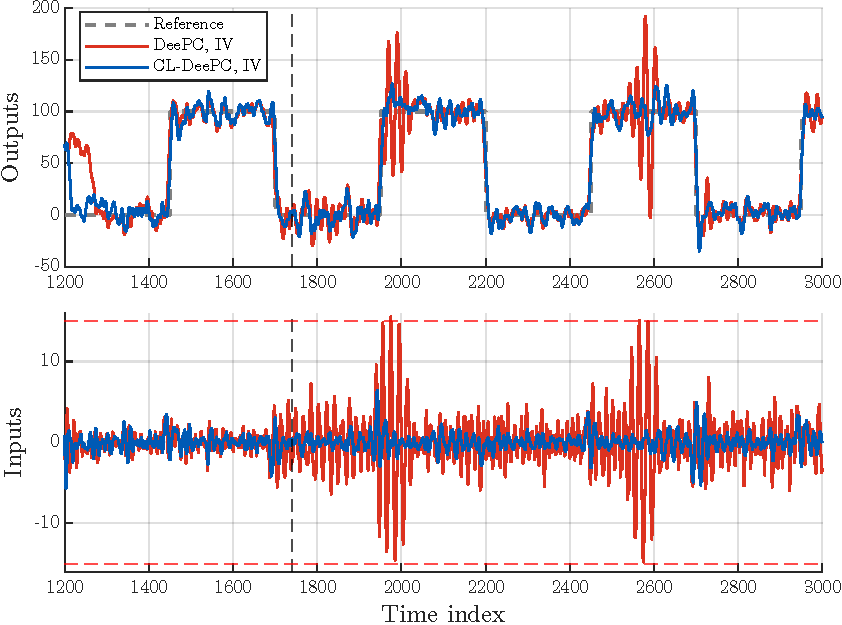
\includegraphics[width=\columnwidth]{results/figures/fig_prob_sol.pdf}    % The printed column  
\caption{Reference tracking by adaptive \ac{DeePC} and \ac{CL-DeePC} using \ac{IVs} with $p=f=20$, and $\bar{N}=539$ for the 5\textsuperscript{th} order system from \cite{Favoreel1999} with $\text{var}(e_k)=0.5$. After $\bar{N}$ samples at the vertical dashed line all input-output data }  % width is 8.4 cm.
\label{fig:CL_Problem_Solution}                                 % Size the figures 
\end{center}                                 % accordingly.
\end{figure}
\section{Equivalence to Closed-loop \acs{SPC}}
This section demonstrates an equivalence between the developed \ac{CL-DeePC} framework and \ac{CL-SPC} as developed in~\cite{Dong2008}. The \ac{CL-SPC} methodology is briefly explained first, based upon which the equivalence is demonstrated thereafter.

\subsection{Closed-loop \ac{SPC}}
To understand this equivalence, consider the data equations \eqref{eq:DataEq1} and \eqref{eq:DataEq2}. Just like \ac{CL-DeePC}, \ac{CL-SPC} uses $s=1$ to avoid closed-loop correlation between inputs and noise\footnote{Treatment of the detrimental effects thereof is reserved for the subsequent section.}, estimating the dynamic matrix $\widetilde{L}_1$ by least squares regression on past data:
\begin{align}\label{eq:CL-SPC-PredMarkov}
\hat{\widetilde{L}}_1 = \left[ \widehat{C\tKp{u}} \; \widehat{D} \; \widehat{C\tKp{y}} \right]=Y_{i_p,1,N}\mathcal{Z}^\top (\Phi_{i,1,N}\mathcal{Z}^\top)\inv,
\end{align}
in which $\mathcal{Z}$ is either $I_N$ or $\Phi_{i,1,N}$ depending on whether an \ac{IV} approach is used or not. Assuming  $\widetilde{A}^p=\mathcal{O}$ as before, estimates of the predictor Markov parameters contained in $\hat{\widetilde{L}}_1$ allow the construction of estimates of $\widetilde{\Gamma}_f\widetilde{K}_p^\mathrm{u}$, $\widetilde{\Gamma}_f\widetilde{K}_p^\mathrm{y}$ and $\widetilde{\mathcal{T}}_f^\mathrm{u}$ (which make up $L_f$), as well as $\tHf$. In line with \eqref{eq:DataEq2} this allows the construction of a predictor as
\begin{align}\label{eq:CL-SPC-pred1}
	\begin{split}
	\datavec{\hat{y}}{\hat{i}_p,f}&= \begin{bmatrix}\widehat{\widetilde{\Gamma}_f\tKp{u}} & \widehat{\widetilde{\mathcal{T}}_f^\mathrm{u}} \end{bmatrix} 
	\begin{bmatrix}
		\datavec{u}{\hat{i},p}\\
		\datavec{u}{\hat{i}_p,f}
	\end{bmatrix}+\\
	&\phantom{=}\mkern8mu\begin{bmatrix}
		\widehat{\widetilde{\Gamma}_f\tKp{y}} & (I_{sl}-\widehat{\widetilde{\mathcal{H}}}_f) \end{bmatrix} 
	\begin{bmatrix}
		\datavec{y}{\hat{i},p}\\
		\datavec{\hat{y}}{\hat{i}_p,f}
	\end{bmatrix}.
	\end{split}
\end{align}
However, this predictor contains the predicted output on both sides of the equation. To solve \eqref{eq:CL-SPC-pred1} for the predicted outputs first make note of the fact that~\cite{Houtzager2012}
\begin{align}\label{eq:MatrixRelations}
	\tHf\inv\begin{bmatrix}
		\widetilde{\Gamma}_f\tKp{u} & \widetilde{\mathcal{T}}_f^\mathrm{u} & \widetilde{\Gamma}_f\tKp{y}
	\end{bmatrix} =
	\begin{bmatrix}
		\Gamma_f\tKp{u} & \mathcal{T}_f^\mathrm{u} & \Gamma_f\tKp{y}
	\end{bmatrix},
\end{align}
as is also visible from the combination of \eqref{eq:DataEq1} and \eqref{eq:DataEq2} for $s=f$. Using \eqref{eq:MatrixRelations} to solve \eqref{eq:CL-SPC-pred1} (which can be done efficiently in a sequential manner as with \ac{CL-DeePC}) yields
\begin{align}\label{eq:CL-SPC-pred2}
		\datavec{\hat{y}}{\hat{i}_p,f}= \begin{bmatrix}\widehat{\Gamma_f\tKp{u}} & \widehat{\Gamma_f\tKp{y}} \end{bmatrix} 
		\begin{bmatrix}
			\datavec{u}{\hat{i},p}\\
			\datavec{y}{\hat{i},p}
		\end{bmatrix}+
		\widehat{\mathcal{T}_f^\mathrm{u}} 
		\datavec{u}{\hat{i}_p,f},
\end{align}
which is in line with \eqref{eq:DataEq1} and is used in a receding horizon optimization-based control framework.

\subsection{Equivalence between \ac{CL-DeePC} and \ac{CL-SPC}}
By comparing \eqref{eq:Sequential1} to \eqref{eq:CL-SPC-pred1} for $f=1$ it can be seen that the building blocks $\tilde{\beta}_k$ and $\tilde{\theta}_k$ in \ac{CL-DeePC} are equal to the estimated predictor Markov parameters from \eqref{eq:CL-SPC-PredMarkov} that are obtained using \ac{CL-SPC}:
\begin{subequations}\label{eq:EquivMarkov}
	\begin{align}
		\tilde{\beta}_k &= \left\{\begin{array}{ll}
			\widehat{C\tilde{A}^{p-k}\tilde{B}}, &\forall k\in\{\mathbb{Z}_{>0}|\;p \geq k \geq 1\}\\
			\widehat{D}, &\text{if } k=p+1
		\end{array}\right.,\label{eq:EquivMarkovInputs}\\
	\tilde{\theta}_k &= \widehat{C\tilde{A}^{p-k}\tilde{B}},\mkern24mu \forall k\in\{\mathbb{Z}_{>0}|\;p \geq k \geq 1\}\label{eq:EquivMarkovOutputs}.
	\end{align}
\end{subequations}
As a result it is clear that there is an equivalence between the constructed matrices in \ac{CL-SPC} and \ac{CL-DeePC} that is succinctly described by
\begin{align}\label{eq:EquivPredictorMatrices}
	\mkern-3mu\begin{bmatrix}
		\widetilde{\mathcal{L}}^\mathrm{u}_f & \widetilde{\mathcal{G}}^\mathrm{u}_f & \widetilde{\mathcal{L}}^\mathrm{y}_f & \left(I_{fl}-\widetilde{\mathcal{G}}^\mathrm{y}_f\right)
	\end{bmatrix}\mkern-3mu=\mkern-3mu\begin{bmatrix}
		\widehat{\widetilde{\Gamma}_f\tKp{u}} & \widehat{\widetilde{\mathcal{T}}_f^\mathrm{u}} & \widehat{\widetilde{\Gamma}_f\tKp{y}} & \widehat{\widetilde{\mathcal{H}}}_f
	\end{bmatrix}\mkern-3mu.
\end{align}
It follows from \eqref{eq:Sequential3}, \eqref{eq:MatrixRelations}, and \eqref{eq:EquivPredictorMatrices} that, likewise,
\begin{align}\label{eq:EquivInnovationMatrices}
	\begin{bmatrix}
		\mathcal{L}^\mathrm{u}_f & \mathcal{G}^\mathrm{u}_f & \mathcal{L}^\mathrm{y}_f
	\end{bmatrix}=\begin{bmatrix}
		\widehat{\Gamma_f\tKp{u}} & \widehat{\mathcal{T}_f^\mathrm{u}} & \widehat{\Gamma_f\tKp{y}}
	\end{bmatrix}.
\end{align}
Moreover,~\eqref{eq:EquivInnovationMatrices} demonstrates that the output predictors~\eqref{eq:Sequential2} and~\eqref{eq:CL-SPC-pred2} of respectively \ac{CL-DeePC} and \ac{CL-SPC} are equivalent. By comparison of the sequential technique from Section~\ref{sec:SequentialSolMethod} to the sequential algorithm of~\cite{Dong2008} it is furthermore possible to see that the two sequential algorithms are indeed equivalent\footnote{Note that direct-feedthrough is not considered in~\cite{Dong2008}, but that an expansion of $B=\tilde{B}+KD$ would yield an algorithm consistent with \ac{CL-DeePC} and~\eqref{eq:MatrixRelations}.}.



\bibliographystyle{elsarticle-harv}%plain       % Include this if you use bibtex 
\bibliography{docs/manuscript/autosam}           % and a bib file to produce the 
                                 % bibliography (preferred). The
                                 % correct style is generated by
                                 % Elsevier at the time of printing.

\appendix
% \section{A summary of Latin grammar}    % Each appendix must have a short title.
% \section{Some Latin vocabulary}         % Sections and subsections are supported  
                                        % in the appendices.
\end{document}